\documentclass[11pt]{book} % or report
\usepackage{amsmath}
\usepackage{amsfonts}
\usepackage{amssymb}
\usepackage{geometry}
\geometry{a4paper, margin=1in}
\usepackage{graphicx}
\usepackage[hidelinks]{hyperref}
\usepackage{amsthm}
\usepackage{tikz}
\usepackage{subcaption}
\usetikzlibrary{positioning}
\usepackage{pgfplots} 
\usepackage[ruled,vlined]{algorithm2e} 
\usepackage{dsfont}
\usepackage{graphicx}
\usepackage{mathdesign}
\usepackage{float}
\usepackage{todonotes} 
\usepackage{empheq}
\usepackage{array}
\usepackage[ruled,vlined]{algorithm2e} 



\setlength{\parindent}{0pt}

% \let\stdsection\section
% \renewcommand\chapter{\newpage\stdsection}

\newcommand\mycommfont[1]{\footnotesize\ttfamily\textcolor{blue}{#1}}
\newcommand\defeq{\stackrel{\mathclap{\normalfont\mbox{def}}}{=}}
\SetCommentSty{mycommfont}

\DeclareMathOperator*{\argmax}{argmax}
\DeclareMathOperator*{\argmin}{argmin}

\newtheorem{theorem}{Theorem}[section]
\newtheorem{lemma}{Lemma}[section]
\newtheorem{definition}{Definition}[section]
\newtheorem{corollary}{Corollary}[section]
\newtheorem{claim}{claim}[section]
\newtheorem{example}{Example}[section]


\newtheorem*{claim*}{Claim}
\newtheorem*{lemma*}{Lemma}
\newtheorem*{corollary*}{Corollary}
\newtheorem*{remark*}{Remark}
\newtheorem*{example*}{Example}
\newtheorem*{examples*}{Examples}
\newtheorem*{definition*}{Definition}



\setcounter{tocdepth}{3}





\begin{document}

\begin{titlepage}
    \begin{center}
     {\huge\bfseries 
     Manifolds \\}
     % ----------------------------------------------------------------
     \vspace{1.5cm}
     {\Large\bfseries Hadar Tal}\\[5pt]
     hadar.tal@mail.huji.ac.il\\[14pt]
      % ----------------------------------------------------------------
     \vspace{2cm}
     {This paper is a summary of the educational materials and lectures from 
     \begin{itemize}
        \item \textbf{Manifolds} by Dr. Julian P. Grossmann, "The Bright Side of Mathematics" 
        \item \textbf{Wikipedia}
        \item \textbf{3Blue1Brown} YouTube channel
     \end{itemize}
     }

     \vfill
    {Winter 2024}
    \end{center}
\end{titlepage}


\frontmatter
\tableofcontents

% * * * * * * * * * * * * * * * * * * * * * * * * 
% * * * * * * * * * * * * * * * * * * * * * * * * 
% * * * * * * * * * * * * * * * * * * * * * * * * 
% * * * * * * * * * * * * * * * * * * * * * * * * 
% * * * * * * * * * * * * * * * * * * * * * * * * 
% * * * * * * * * * * * * * * * * * * * * * * * * 
% * * * * * * * * * * * * * * * * * * * * * * * * 
% * * * * * * * * * * * * * * * * * * * * * * * * 
% * * * * * * * * * * * * * * * * * * * * * * * * 
% * * * * * * * * * * * * * * * * * * * * * * * * 
% * * * * * * * * * * * * * * * * * * * * * * * * 
% * * * * * * * * * * * * * * * * * * * * * * * * 
% * * * * * * * * * * * * * * * * * * * * * * * * 
% * * * * * * * * * * * * * * * * * * * * * * * * 
% * * * * * * * * * * * * * * * * * * * * * * * * 
% * * * * * * * * * * * * * * * * * * * * * * * * 
% * * * * * * * * * * * * * * * * * * * * * * * * 
% * * * * * * * * * * * * * * * * * * * * * * * * 
% * * * * * * * * * * * * * * * * * * * * * * * * 

\mainmatter

\chapter{Metric space and complete metric space}

\begin{definition}{\textbf{Metric Space}} \\
    A metric space is a set \( X \) equipped with a metric, which is a function that defines a distance between each pair of elements in \( X \), satisfying the following properties for all \( x, y, z \in X \):
    \begin{enumerate}
        \item Non-negativity: \( d(x, y) \geq 0 \) and \( d(x, y) = 0 \) if and only if \( x = y \)
        \item Symmetry: \( d(x, y) = d(y, x) \)
        \item Triangle inequality: \( d(x, y) + d(y, z) \geq d(x, z) \)
    \end{enumerate}
\end{definition}

\( \textbf{Inner Product Space vs Metric Space} \)
\begin{itemize}
    \item An inner product space is a vector space equipped with an inner product, which is a function that associates each pair of vectors with a scalar.
    \item A metric space is a set equipped with a metric, which is a function that defines a distance between each pair of elements in the set.
    \item Every inner product space is a metric space, but not every metric space is an inner product space.
        \begin{example*}
            Each inner product space must satisfy the Parallelogram Law, which states that for all \( u, v \) in the space, \( 2\|u\|^2 + 2\|v\|^2 = \|u + v\|^2 + \|u - v\|^2 \).
            A clasic example of a metric space that is not an inner product space is the space of continuous functions on the interval \([0, 1]\) with the metric \( d(f, g) = \max_{x \in [0, 1]} |f(x) - g(x)| \).
        \end{example*}
\end{itemize}

\begin{definition}{ \textbf{Open $\epsilon$-ball} } \\
    Let \( (X, d) \) be a metric space and \( x \in X \). \\
    The open \(\varepsilon\)-ball centered at \( x \) is the set \(  B(x, \varepsilon) = \{ y \in X : d(x, y) < \varepsilon \} \).
\end{definition}

\begin{definition}{ \textbf{Open set} (metric space) } \\
    A subset \( U \) of a metric space \( (X, d) \) is open if for every point \( x \in U \), 
    there exists an open \(\varepsilon\)-ball centered at \( x \) that is contained in \( U \).
\end{definition}

\begin{definition}{\textbf{Convergence of a sequence}} \\
    A sequence \( (x_n) \) in a metric space \( (X, d) \) is said to \emph{converge} to a limit \( a \in X \) if, for every positive real number \( \varepsilon > 0 \),
    there exists a positive integer \( N \) such that for all positive integers \( n \geq N \), \( x_n \in B_{\varepsilon}(a) \).
\end{definition}

\begin{definition}{\textbf{Cauchy Sequence}} \\
    In a metric space \( (X, d) \), a sequence \( \{x_1, x_2, x_3, \ldots\} \) is said to be \emph{Cauchy} if, for every positive real number \( \varepsilon > 0 \),
     there exists a positive integer \( N \) such that for all positive integers \( m, n > N \), the distance
    \[ d(x_m, x_n) < \varepsilon. \]
\end{definition}

\begin{figure}[H]
    \begin{subfigure}{0.5\textwidth}
        \centering
        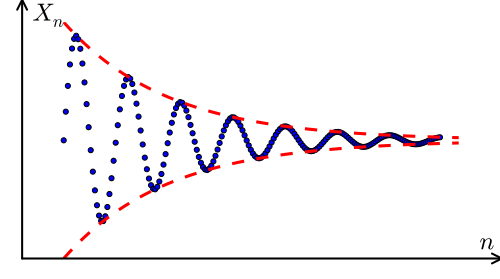
\includegraphics[width=0.45\textwidth]{Figs/Cauchy_sequence_illustration.png}
        \caption{The plot of a Cauchy sequence \( (x_n) \) shown in blue, as \( x_n \) versus \( n \). If the space is complete, then the sequence has a limit.}
    \end{subfigure}
    \hfill
    \begin{subfigure}{0.45\textwidth}
        \centering
        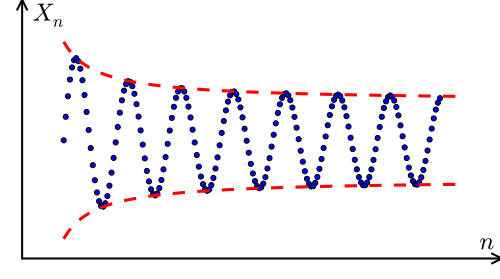
\includegraphics[width=0.5\textwidth]{Figs/Cauchy_sequence_illustration2.png}
        \caption{A sequence that is not Cauchy. The elements of the sequence do not get arbitrarily close to each other as the sequence progresses.}
    \end{subfigure}
    \caption{Cauchy Sequence}
\end{figure}

\begin{definition}{\textbf{Complete Metric Space}} \\
    A metric space is complete if every Cauchy sequence in the space converges to a limit in the space.
\end{definition}

\subsection{Hilbert Space}

\begin{definition}{\textbf{Hilbert Space}} \\
    A \emph{Hilbert space} is a complete inner product space. That is, it is an inner product space \( \mathcal{H} \) that 
    is also a complete metric space with respect to the metric induced by its inner product. 
    The metric is given by \( d(x,y) = \sqrt{\langle x-y, x-y \rangle} \) for all \( x, y \in \mathcal{H} \).
\end{definition}
    
A Hilbert space generalizes the notion of Euclidean space to an infinite-dimensional context. 
In a Hilbert space, one can still use concepts like angle, orthogonality, and projection, which are crucial in many areas of mathematics and physics. 
Completeness is a key feature of Hilbert spaces, meaning that every Cauchy sequence in the space converges to a limit within the space. 
    

% * * * * * * * * * * * * * * * * * * * * * * * *
% * * * * * * * * * * * * * * * * * * * * * * * *
% * * * * * * * * * * * * * * * * * * * * * * * *
% * * * * * * * * * * * * * * * * * * * * * * * *
% * * * * * * * * * * * * * * * * * * * * * * * *
% * * * * * * * * * * * * * * * * * * * * * * * *
% * * * * * * * * * * * * * * * * * * * * * * * *


\chapter{Topological Space}

\begin{definition}{\textbf{Topology}} \\
A topology \( \mathcal{T} \) on a set \( X \) is a collection of subsets of  \( X \) that satisfy the following properties:
\begin{enumerate}
    \item \( \emptyset, X \in \mathcal{T} \).
    \item The intersection of any finite number of sets is in \( \mathcal{T} \) - \\ 
    \( U_1, U_2, \ldots, U_n \in \mathcal{T} \) implies \( \bigcap_{i=1}^n U_i \in \mathcal{T} \).
    \item The union of any number of sets (finite or infinite) is in \( \mathcal{T} \) - \\
    \( U_\alpha \in \mathcal{T} \) for all \( \alpha \) in some index set \( A \) implies \( \bigcup_{\alpha \in A} U_\alpha \in \mathcal{T} \).
\end{enumerate}
\end{definition}

\begin{definition}{\textbf{Topological Space}} \\
A topological space is a pair \( (X, \mathcal{T}) \) consisting of a set \( X \) and a topology \( \mathcal{T} \) on \( X \).
\end{definition}

A metric space \( (X, d) \) induces a topology on \( X \) by defining the open sets to be the unions of open \( \varepsilon \)-balls centered at each point in \( X \). 

\begin{example*}
Examples of topological spaces:
\begin{enumerate}
    \item \( X = {1, 2, 3} \) with the topology \( T = \{\varnothing , \{1\}, \{1, 2\}, \{1, 2, 3\} \} \).
    \item Given any set $X$, \textbf{the discrete topology} on $X$ is the power set of $X$ - $\mathcal{T} = P(X)$ and is the largest possible topology on $X$.
    \item \textbf{The indiscrete topology} on $X$ is $\mathcal{T} = \{\emptyset, X\}$ and is the smallest possible topology on $X$ - 
    $\forall \mathcal{T}$, $\{\emptyset, X\} \subseteq \mathcal{T} \subseteq P(X)$.
    \item The real line \( \mathbb{R} \) with the standard topology.
    \item The set of integers \( \mathbb{Z} \) with the discrete topology.
    \item The set of real numbers \( \mathbb{R} \) with the lower limit topology.
\end{enumerate}
\end{example*}

\begin{definition}{\textbf{Open Set (topological space)}} \\
    A subset \( U \) of a topological space \( (X, \mathcal{T}) \) is open if \( U \in \mathcal{T} \).
\end{definition}

\begin{definition}{\textbf{Metrizible Space}} \\
    A topological space \( (X, \mathcal{T}) \) is metrizable if there exists a metric \( d \) on \( X \) such that 
    the topology induced by \( d \) is equal to \( \mathcal{T} \).
\end{definition}

% * * * * * * * * * * * * * * * * * * * * * * * *
% * * * * * * * * * * * * * * * * * * * * * * * *
% * * * * * * * * * * * * * * * * * * * * * * * *
% * * * * * * * * * * * * * * * * * * * * * * * *
% * * * * * * * * * * * * * * * * * * * * * * * *
% * * * * * * * * * * * * * * * * * * * * * * * *
% * * * * * * * * * * * * * * * * * * * * * * * *


\chapter{Interior, exterior, boundary, and accumulation points}

Let \( (X, \mathcal{T}) \) be a topological space , and \( S \subseteq X \) (it can be an open set but it not necessarily has to be).

\begin{definition}{\textbf{Interior point}} \\
    A point \( p \in S \) is an interior point of \( S \) if there exists an open set \( U \) such that \( p \in U \subseteq S \).
\end{definition}

\begin{definition}{\textbf{Exterior point}} \\
    A point \( p \in X \) is an exterior point of \( S \) if there exists an open set \( U \) such that \( p \in U \subseteq X \setminus S \).
\end{definition}

\begin{definition}{\textbf{Boundary point}} \\
    A point \( p \in X \) is a boundary point of \( S \) if for every open set \( U \) containing \( p \), both \( U \cap S \) and \( U \cap (X \setminus S) \) are non-empty.
\end{definition}

\begin{definition}{\textbf{Accumulation (limit) point}} \\
    A point \( p \in X \) is an accumulation point of \( S \) if for every open set \( U \) containing \( p \), the set \( ( U \setminus \{p\} ) \cap S \) is non-empty.
\end{definition}

\begin{figure}[H]
    \begin{subfigure}{0.24\textwidth}
        \centering
        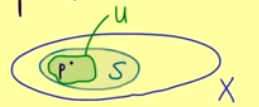
\includegraphics[width=\textwidth]{Figs/interior.png}
        \caption{Interior point}
    \end{subfigure}
    \begin{subfigure}{0.24\textwidth}
        \centering
        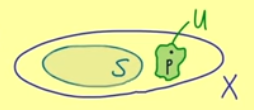
\includegraphics[width=\textwidth]{Figs/exterior.png}
        \caption{Exterior point}
    \end{subfigure}
    \begin{subfigure}{0.24\textwidth}
        \centering
        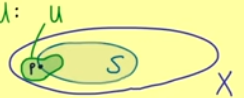
\includegraphics[width=\textwidth]{Figs/boundary.png}
        \caption{Boundary point}
    \end{subfigure}
    \begin{subfigure}{0.24\textwidth}
        \centering
        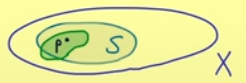
\includegraphics[width=\textwidth]{Figs/accumulation.png}
        \caption{Accumulation point}
    \end{subfigure}
    \caption{Interior, exterior, and boundary points of a set}
\end{figure}


\begin{definition}{\textbf{Interior of a set}} \\
    The interior of a set \( S \), denoted by \( \text{int}(S) \) or \( S^\circ \), is the set of all interior points of \( S \).
    \begin{equation*}
        S^\circ = \{ p \in S : p \text{ is an interior point of } S \}
    \end{equation*}
\end{definition}


\begin{definition}{\textbf{Exterior of a set}} \\
    The exterior of a set \( S \), denoted by \( \text{ext}(S) \), is the set of all exterior points of \( S \).
    \begin{equation*}
        \text{ext}(S) = \{ p \in X : p \text{ is an exterior point of } S \}
    \end{equation*}
\end{definition}

\begin{definition}{\textbf{Boundary of a set}} \\
    The boundary of a set \( S \), denoted by \( \text{bd}(S) \) or \( \partial S \), is the set of all boundary points of \( S \).
    \begin{equation*}
        \partial(S) = \{ p \in X : p \text{ is a boundary point of } S \}
    \end{equation*}
\end{definition}

The boundary of a set \( S \) consists of all points that are either in the interior of \( S \) or in the exterior of \( S \).


\begin{definition}{\textbf{Derived set} (derivative of a set)} \\
    The derived set of a set \( S \), denoted by \( S' \), is the set of all accumulation points of \( S \).
    \begin{equation*}
        S' = \{ p \in X : p \text{ is an accumulation point of } S \}
    \end{equation*}
\end{definition}

\begin{definition}{\textbf{Closure of a set}} \\
    The closure of a set \( S \), denoted by \( \overline{S} \), is the set of all points in \( X \) that are either in \( S \) or are accumulation points of \( S \).
    \begin{equation*}
        \overline{S} = S \cup S'
    \end{equation*}
\end{definition}


\begin{example*}
    X = \( \mathbb{R} \) ,  \( \mathbb{T} = \{ \emptyset, \mathbb{R} \} \cup \{ ( a, \infty ) : a \in \mathbb{R} \} \) is a topology on \( \mathbb{R} \). \\
    S = \( (0, 1) \) is not an open set, and do not have any interior points. \\
    $ X \setminus S = (-\infty, 0] \cup [1, \infty) \Rightarrow  \text{ext}(S) = (1, \infty) \Rightarrow \partial S =  [-\infty, 1)  $.)
    
\end{example*}

\begin{definition}{\textbf{Closed set}} \\
    Let \( (X, \mathcal{T}) \) be a topological space. A set \( S \subseteq X \) is closed if any of the following equivalent conditions hold:
    \begin{itemize}
        \item A set \( S \) is closed if it contains all of its boundary points.
        \item A set \( S \) is closed if its complement \( X \setminus S \) is open.
        \item A set \( S \) is closed if it is equal to its closure \( \overline{S} \).
    \end{itemize}
\end{definition}

% * * * * * * * * * * * * * * * * * * * * * * * *
% * * * * * * * * * * * * * * * * * * * * * * * *
% * * * * * * * * * * * * * * * * * * * * * * * *
% * * * * * * * * * * * * * * * * * * * * * * * *
% * * * * * * * * * * * * * * * * * * * * * * * *
% * * * * * * * * * * * * * * * * * * * * * * * *
% * * * * * * * * * * * * * * * * * * * * * * * *

\chapter{Hausdorff space}

\begin{definition}{\textbf{Open neighbothood of a point}} \\
    An open neighborhood of a point \( a \) in a topological space \( (X, \mathcal{T}) \) is an open set containing \( a \).
\end{definition}

\begin{definition}{ \textbf{Convergence of a sequence} } \\
    A sequence \( (x_n) \) in a topological space \( (X, \mathcal{T}) \) is said to converge to a limit \( a \in X \) 
    if for every open neighborhood \( U \) of \( a \), there exists a positive integer \( N \) such that for all positive integers \( n \geq N \), \( x_n \in U \).
\end{definition}

Note that there can be multiple limits of a sequence in a topological space, and the limit need not be unique.

\begin{example*}
    X = \( \mathbb{R} \) ,  \( \mathbb{T} = \{ \emptyset, \mathbb{R} \} \cup \{ ( a, \infty ) : a \in \mathbb{R} \} \) is a topology on \( \mathbb{R} \). \\
    \( (a_n)_{n \in \mathbb{N}} = (\frac{1}{n})_{n \in \mathbb{N}} \) converges to 0, but also to any \( a \in (0, \infty) \).
    \begin{itemize}
        \item It converges to 0 - every open neighborhood of 0 looks like \( (a, \infty) \) for some \( a < 0 \) so \( \frac{1}{n} \in (a, \infty) \).
        \item It converges to -1 - every open neighborhood of -1 looks like \( (a, \infty) \) for some \( a < -1 \) so \( \frac{1}{n} \in (a, \infty) \).
        \item The same argument can be made for any \( a \in (-\infty, 0] \).
    \end{itemize}
\end{example*}

\begin{definition}{\textbf{Hausdorff Space}} \\
    A topological space \( (X, \mathcal{T}) \) is a Hausdorff space if for every pair of distinct points \( x, y \in X \), there exist open sets \( U \) and \( V \) such that \( x \in U \), \( y \in V \), and \( U \cap V = \emptyset \).
\end{definition}

\begin{figure}[H]
    \centering
    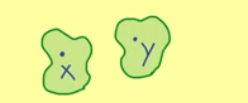
\includegraphics[width=0.3\textwidth]{Figs/hausdorff_space.png}
    \caption{Hausdorff space}
\end{figure}

In a Hausdorff space, every pair of distinct points can be separated by disjoint open sets.

% * * * * * * * * * * * * * * * * * * * * * * * *
% * * * * * * * * * * * * * * * * * * * * * * * *
% * * * * * * * * * * * * * * * * * * * * * * * *
% * * * * * * * * * * * * * * * * * * * * * * * *
% * * * * * * * * * * * * * * * * * * * * * * * *
% * * * * * * * * * * * * * * * * * * * * * * * *
% * * * * * * * * * * * * * * * * * * * * * * * *


\chapter{Quotient space}

\begin{definition}{\textbf{Projective space}} \\
    The projective space \( \mathbf{P}^n (\mathbb{R}) \) is the set of all lines passing through the origin in \( \mathbb{R}^{n+1} \).
    It can be thought of as the space of all one-dimensional subspaces of \( \mathbb{R}^{n+1} \).
\end{definition}

\begin{figure}[H]
    \centering
    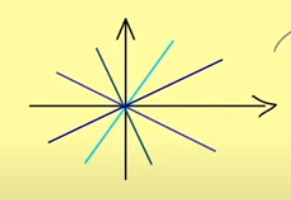
\includegraphics[width=0.3\textwidth]{Figs/projective_space_2d.png}
    \caption{The projective space \( \mathbf{P}^1 \) - all the lines passing through the origin in \( \mathbb{R}^2 \) }
\end{figure}

The directions define a set, and we want to create a topological space for this set.

\begin{definition}{\textbf{Equivalence relation}} \\
    An equivalence relation on a set \( X \) is a relation \( \sim \) that satisfies the following properties for all \( x, y, z \in X \):
    \begin{enumerate}
        \item Reflexivity: \( x \sim x \)
        \item Symmetry: \( x \sim y \) implies \( y \sim x \)
        \item Transitivity: \( x \sim y \) and \( y \sim z \) implies \( x \sim z \)
    \end{enumerate}
\end{definition}

\begin{definition}{\textbf{Equivalence class}} \\
    Let \( X \) be a set and \( \sim \) be an equivalence relation on \( X \). \\
    The equivalence class of \( x \) with respect to \( \sim \) is
    \begin{equation*}
        [x]_\sim = \{ y \in X : y \sim x \}
    \end{equation*}
\end{definition}

\begin{definition}{\textbf{Quotient set}} \\
    Let \( X \) be a set and \( \sim \) be an equivalence relation on \( X \). \\
    The quotient set \( X / \sim \) is defined as 
    \begin{equation*}
        X/\sim \quad = \{ [x]_\sim : x \in X \}
    \end{equation*}
\end{definition}

\begin{definition}{\textbf{Quotient map (Canonical projection)}} \\
    Let \( X \) be a set and \( \sim \) be an equivalence relation on \( X \). \\
    The canonical projection is a function:
    \begin{equation*}
        q: X \to X/\sim \quad \text{such that} \quad q(x) = [x]_\sim
    \end{equation*}
\end{definition}

\begin{definition}{\textbf{Quotient Topology}} \\
    Let \( X , \mathcal{T} \) be a topological space, \( \sim \) be an equivalence relation on \( X \) and \( q: X \to X/\sim \) be the canonical projection. \\
    The quotient topology \( \hat{\mathcal{T}} \) on \( X/\sim \) is defined as
    \begin{equation*}
        \hat{\mathcal{T}} = \{ U \subseteq X/\sim \quad : q^{-1}(U) \in \mathcal{T} \}
    \end{equation*}
\end{definition}

\begin{figure}[H]
    \centering
    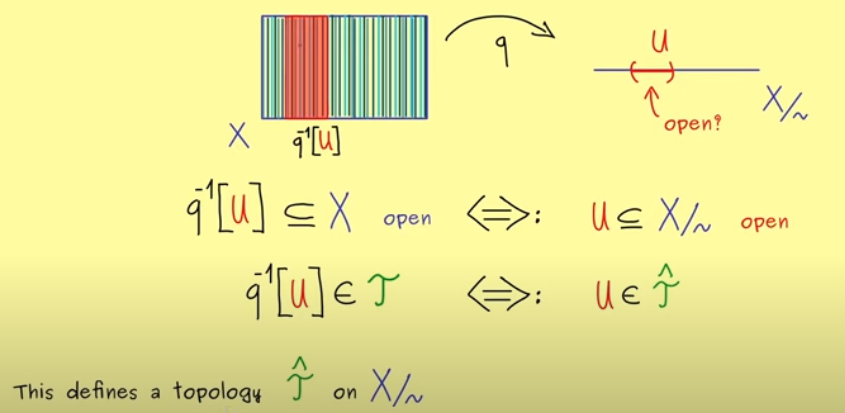
\includegraphics[width=0.8\textwidth]{Figs/quotient_topology.png}
    \caption{Quotient Topology}
\end{figure}

\begin{example*} A classic example of a quotient space is the \textbf{mobius strip}, which is constructed by taking a rectangular strip of paper, 
    giving one end a half-twist, and then gluing the two ends together. The mobius strip is a non-orientable surface, 
    meaning that it does not have a consistent notion of "left" and "right" across the entire surface. 
    The mobius strip is a quotient space of a square, where the opposite edges of the square are identified in a specific way.
    Formally, 
    \begin{align*}
        X = [0, 1] \times (-1, 1) \quad \text{and} \quad &\sim \text{ is the equivalence relation that identifies the points} \\
        (0, y) &\sim (1, -y) \quad \text{for all} \quad y \in (-1, 1).
    \end{align*}
\end{example*}

\begin{figure}[H]
    \centering
    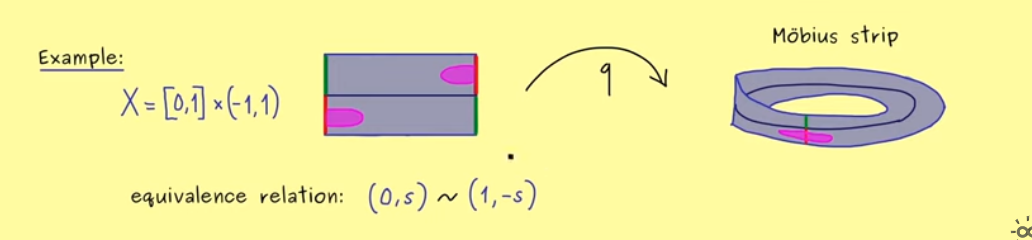
\includegraphics[width=0.8\textwidth]{Figs/mobius_strip.png}
    \caption{Mobius Strip}
\end{figure}

% * * * * * * * * * * * * * * * * * * * * * * * *
% * * * * * * * * * * * * * * * * * * * * * * * *
% * * * * * * * * * * * * * * * * * * * * * * * *
% * * * * * * * * * * * * * * * * * * * * * * * *
% * * * * * * * * * * * * * * * * * * * * * * * *
% * * * * * * * * * * * * * * * * * * * * * * * *
% * * * * * * * * * * * * * * * * * * * * * * * *


\chapter{Projective Space}

So far we have seen the transition from topological space to quotient space:
\begin{equation*}
    (X, \mathcal{T}) \to (X/\sim, \hat{\mathcal{T}})
\end{equation*}

Recall that the projective space \( \mathbf{P}^n (\mathbb{R}) \) is the set of all lines passing through the origin in \( \mathbb{R}^{n+1} \).

\begin{definition}{\textbf{Sphere}} \\
    The sphere \( S^n \) is the set of all points in \( \mathbb{R}^{n+1} \) that are at a fixed distance of 1 from the origin.
    \begin{equation*}
        S^n = \{ x \in \mathbb{R}^{n+1} : \|x\|_2 = 1 \}
    \end{equation*}
\end{definition}

\begin{definition}{\textbf{The Projective Space as quotient space}} \\
    The projective space \( \mathbf{P}^n (\mathbb{R}) \) can be constructed as a quotient space of the sphere \( S^n \) by identifying antipodal points.
    \begin{equation*}
        \mathbf{P}^n (\mathbb{R}) = S^n / \sim
    \end{equation*}
    where the equivalence relation \( \sim \) is defined as
    \begin{equation*}
        x \sim y \quad \text{if} \quad x = y \quad \text{or} \quad x = -y
    \end{equation*}
\end{definition}

\begin{figure}[H]
    \centering
    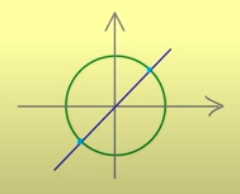
\includegraphics[width=0.3\textwidth]{Figs/projective_space.png}
    \caption{Projective Space as a quotient space}
\end{figure}

The sphere \( S^n \) is a hausdorff space, and the projective space \( \mathbf{P}^n (\mathbb{R}) \) is also a hausdorff space.
But in general, the quotient space of a hausdorff space is not necessarily a hausdorff space.
Take \( [x]_\sim, [y]_\sim \in \mathbf{P}^n (\mathbb{R}) \) such that \( [x]_\sim \neq [y]_\sim \Rightarrow x \neq y \) and \( x \neq -y \) .

\begin{figure}[H]
    \begin{subfigure}{\textwidth}
        \centering
        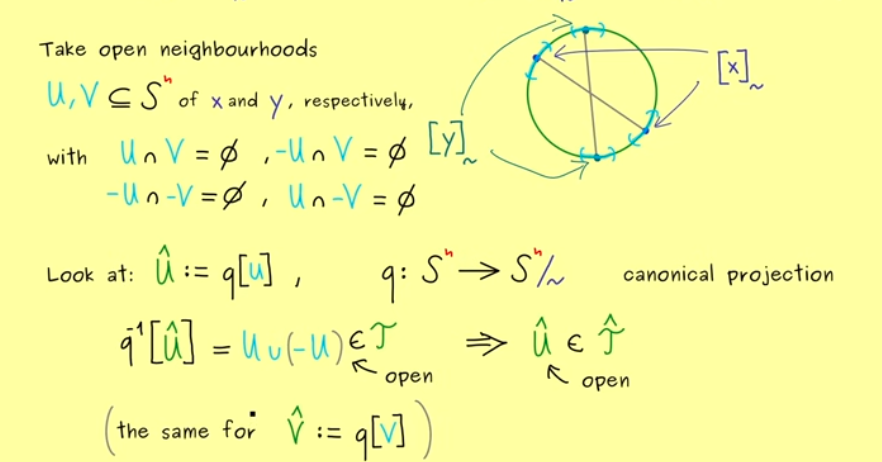
\includegraphics[width=\textwidth]{Figs/projective_space_is_hausdorff.png}
    \end{subfigure}
    \begin{subfigure}{\textwidth}
        \centering
        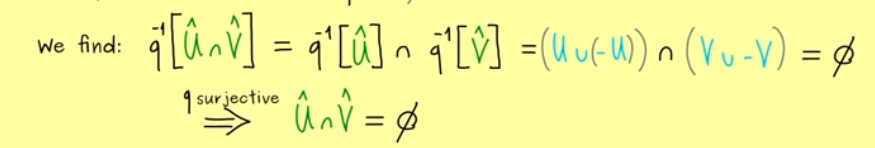
\includegraphics[width=\textwidth]{Figs/projective_space_is_hausdorff2.png}
    \end{subfigure}
    \caption{Projective Space as a hausdorff space}
\end{figure}

% * * * * * * * * * * * * * * * * * * * * * * * *
% * * * * * * * * * * * * * * * * * * * * * * * *
% * * * * * * * * * * * * * * * * * * * * * * * *
% * * * * * * * * * * * * * * * * * * * * * * * *
% * * * * * * * * * * * * * * * * * * * * * * * *
% * * * * * * * * * * * * * * * * * * * * * * * *
% * * * * * * * * * * * * * * * * * * * * * * * *

\chapter{First Countable Space}

\begin{definition}{\textbf{First Countable Space}} \\
    A topological space \( (X , \mathcal{T}) \) is said to be \emph{first countable} if at every point \( x \) in \( X \), 
    there exists a countable basis for the neighborhoods of \( x \). That is: \\ 
    \begin{align*}
        &\forall x \in X, \quad \exists \{ U_i \}_{i=1}^{\infty} \quad \text{such that} \quad \forall i \in \mathbb{N} \quad x \in U_i \\
        &\text{and} \quad \forall V \in \mathcal{T} \quad \text{such that} \quad x \in V , \quad \exists i \quad \text{such that} \quad U_i \subseteq V
    \end{align*}
    The countable set of open sets \( \{ U_i \}_{i=1}^{\infty} \) is called a \textbf{local basis} at \( x \).
\end{definition}

\begin{examples*} of first countable spaces:
    \begin{itemize}
        \item \textbf{Metric Spaces}: Every metric space is first countable. 
        The local basis at any point \( x \) in a metric space can be chosen as the collection of open balls centered 
        at \( x \) with radii \( 1/n \), where \( n \) is a positive integer.

        \item \textbf{Subspaces of Metric Spaces}: Any subspace of a metric space inherits the first countability. 
        If \( Y \) is a subspace of a metric space \( X \), then the local bases in \( Y \) can be constructed using 
        the intersections of open balls in \( X \) with \( Y \).

        \item \textbf{Euclidean Spaces \( \mathbb{R}^n \)}: The Euclidean space with its standard topology, 
        which is generated by the open balls, is first countable.

        \item \textbf{The Space of Rational Numbers \( \mathbb{Q} \)}: As a subspace of the real line \( \mathbb{R} \), 
        which is a metric space, the space of rational numbers \( \mathbb{Q} \) is first countable.
    \end{itemize}
\end{examples*}

\chapter{Second Countable Space}

\begin{definition}{\textbf{Basis}} \\
    A basis for a topological space \( (X, \mathcal{T}) \) is a collection \( \mathcal{B} \subseteq \mathcal{T} \) of open sets 
    such that every open set in \( \mathcal{T} \) can be written as a union of sets in \( \mathcal{B} \).
\end{definition}

\begin{examples*} of basis:
    \begin{itemize}
        \item \( \mathcal{B} = \mathcal{T} \) is a basis for \( \mathcal{T} \).
        \item If \( \mathcal{T} \) is discrete, then \( \mathcal{B} = \{ \{ x \} : x \in X \} \) is a basis for \( \mathcal{T} \).
        \item Let \( (X, \mathcal{T}) \) be a topological space induced by a metric space \( (X, d) \). \\
            Then \( \mathcal{B} = \{ B_\varepsilon(x) : x \in X, \varepsilon > 0 \} \) is a basis for \( \mathcal{T} \).
        \item \( \mathbb{R}^n \) with the standard topology (defined by the Euclidean metric) has a basis of open balls.
            Then \( \mathcal{B} = \{ B_{\varepsilon}(x) : x \in \mathbb{Q}^n, \varepsilon \in \mathbb{Q}, \varepsilon > 0 \} \) is a basis for \( \mathcal{T} \).
            Eventhought the space is uncountable, the basis has a countable number of elements.
    \end{itemize}
\end{examples*}

\begin{definition}{\textbf{Second Countable Space}} \\
    A topological space \( (X, \mathcal{T}) \) is second countable if there exists a countable basis for \( \mathcal{T} \).
\end{definition}


\begin{examples*} of second countable spaces:
    \begin{itemize}
        \item Any finite or countable discrete space.
        \item The real line \( \mathbb{R} \) with the standard topology.
        \item The Euclidean space \( \mathbb{R}^n \) with the standard topology.
        \item The space of continuous functions \( C([0, 1]) \) with the topology of uniform convergence.
    \end{itemize}
\end{examples*}

\begin{examples*} of spaces that are not second countable:
    \begin{itemize}
        \item Consider an uncountable set (like \( \mathbb{R} \)) with the discrete metric (the distance between each pair of distinct
         points is 1, and the distance between a point and itself is 0). 
         In this metric space, every singleton set is open, therefore to have a base for the topology, we need to include every singleton,
         which is an uncountable number.
    \end{itemize}
    
\end{examples*}

\begin{definition}{\textbf{The space of continuous functions with the topology of uniform convergence}} \\
    Let \( C([0, 1]) \) be the space of continuous functions on the interval \( [0, 1] \). \\
    The topology of uniform convergence on \( C([0, 1]) \) is defined by the basis
    \begin{equation*}
        \mathcal{B} = \{ B_{\varepsilon}(f) : f \in C([0, 1]), \varepsilon > 0 \}
    \end{equation*}
    where \( B_{\varepsilon}(f) = \{ g \in C([0, 1]) : \| f - g \|_{\infty} < \varepsilon \} \).
\end{definition}

\begin{figure}[H]
    \centering
    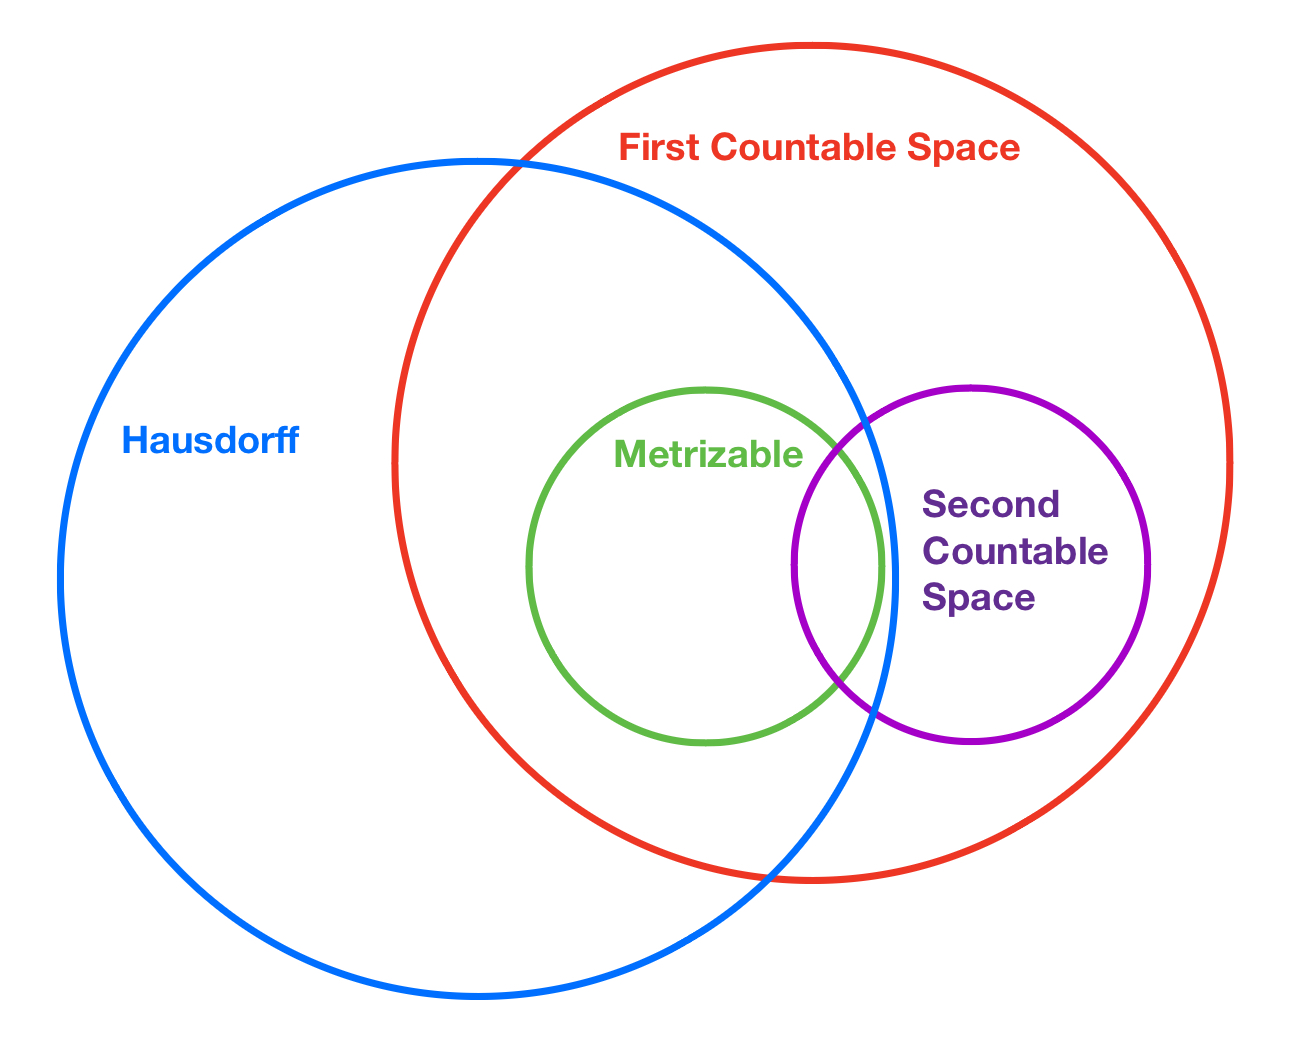
\includegraphics[width=0.5\textwidth]{Figs/topological_spaces_diagram.jpeg}
    \caption{Venn diagram of topological spaces - Metrizable, Hausdorff, First Countable, Second Countable}
\end{figure}


% * * * * * * * * * * * * * * * * * * * * * * * *
% * * * * * * * * * * * * * * * * * * * * * * * *
% * * * * * * * * * * * * * * * * * * * * * * * *
% * * * * * * * * * * * * * * * * * * * * * * * *
% * * * * * * * * * * * * * * * * * * * * * * * *
% * * * * * * * * * * * * * * * * * * * * * * * *
% * * * * * * * * * * * * * * * * * * * * * * * *

\chapter{Continuity}

Recall the definition of continuity of a function in $R^n$:
\begin{definition*}{\textbf{Continuity of a function}} \\
    A function \( f: \mathbb{R}^n \to \mathbb{R} \) is continuous at a point \( x \in \mathbb{R}^n \) 
    if for every \( \varepsilon > 0 \), there exists \( \delta > 0 \) such that for all \( y \in \mathbb{R}^n \) with
     \( \| x - y \|_2 < \delta \), we have \( \| f(x) - f(y) \|_2 < \varepsilon \).
\end{definition*}

or equivalently, in term of sequences:
\begin{definition*}{\textbf{Continuity of a function (sequence definition)}} \\
    A function \( f: \mathbb{R}^n \to \mathbb{R} \) is continuous at a point \( x \in \mathbb{R}^n \) 
    if for every sequence \( (x_k) \) in \( \mathbb{R}^n \) such that \( x_k \to x \), we have \( f(x_k) \to f(x) \).
\end{definition*}

Now, we extend the definition of continuity to topological spaces.

\begin{definition}{\textbf{Continuity of a function at a point (topological space)}} \\
    Let \( (X, \mathcal{T}_X) \) and \( (Y, \mathcal{T}_Y) \) be topological spaces. \\
    A function \( f: X \to Y \) is continuous at a point \( x \in X \) if for every neighborhood \( V \) of \( f(x) \) in \( Y \),
    there exists a neighborhood \( U \) of \( x \) in \( X \) such that \( f(U) \subseteq V \).
\end{definition}

\begin{figure}[H]
    \centering
    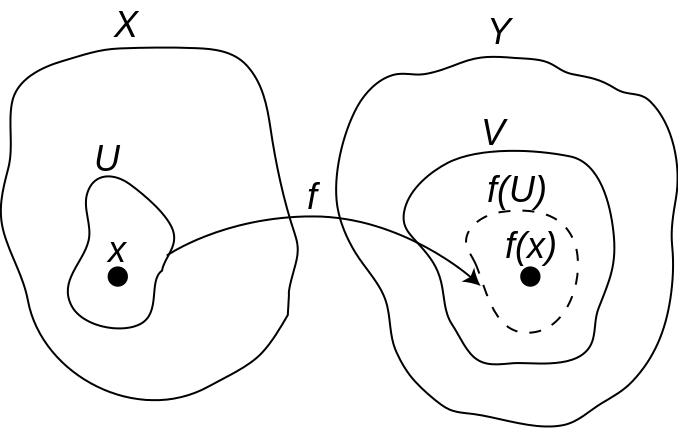
\includegraphics[width=0.4\textwidth]{Figs/continuity_topology.png}
    \caption{Continuity of a function at a point} 
\end{figure}


\begin{definition}{\textbf{Continuity of a function (topological space)}} \\
    Let \( (X, \mathcal{T}_X) \) and \( (Y, \mathcal{T}_Y) \) be topological spaces. \\
    A function \( f: X \to Y \) is continuous if for every open set \( U \in \mathcal{T}_Y \), \( f^{-1}(U) \in \mathcal{T}_X \) \\
    (the preimage of an open set is open).
\end{definition}

\begin{figure}[H]
    \centering
    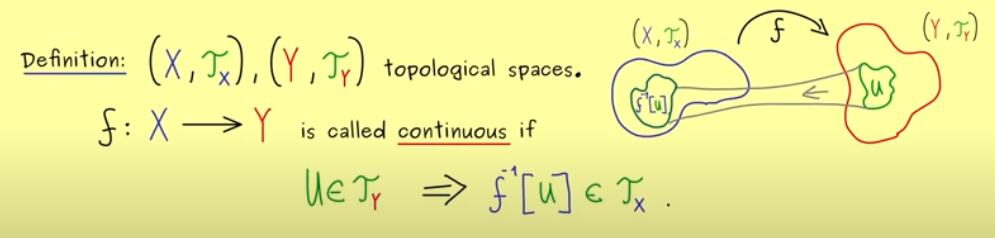
\includegraphics[width=\textwidth]{Figs/continuity.png}
    \caption{Continuity of a function}    
\end{figure}

In term of sequences:

\begin{definition}{\textbf{Sequentially continuous function (topological space)}} \\
    Let \( (X, \mathcal{T}_X) \) and \( (Y, \mathcal{T}_Y) \) be topological spaces. \\
    A function \( f: X \to Y \) is sequentially continuous if for every \( x \in X \) and every sequence 
    \( (x_n)_{n \in \mathbb{N}} \subseteq X \) such that \( x_n \to x \), \( (f(x_n))_{n \in \mathbb{N}} \subseteq Y \) convergent 
    with \( (f(x_n))_{n \in \mathbb{N}} \to f(x) \).
\end{definition}

\begin{figure}[H]
    \centering
    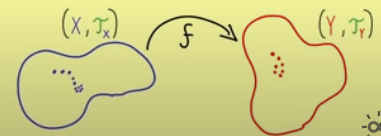
\includegraphics[width=0.4\textwidth]{Figs/sequentially_continues_function.png}
    \caption{Sequentially continuous function}
\end{figure}

\begin{theorem}{\textbf{Continuity vs Sequential Continuity}} \\
    Let \( (X, \mathcal{T}_X) \) and \( (Y, \mathcal{T}_Y) \) be topological spaces and \( f: X \to Y \) be a function. \\
    \begin{align*}
        \text{f is continuous} &\Rightarrow \text{f is sequentially continuous} \\
        \text{f is continuous} &\nLeftarrow \text{f is sequentially continuous}
    \end{align*}
\end{theorem}

\begin{theorem}{\textbf{Continuity vs Sequential Continuity in First Countable Spaces}} \\
    Let \( (X, \mathcal{T}_X) \) and \( (Y, \mathcal{T}_Y) \) be First Countable spaces and \( f: X \to Y \) be a function. Then 
    \begin{align*}
        \text{f is continuous} &\Leftrightarrow \text{f is sequentially continuous}
    \end{align*}
\end{theorem}

\begin{examples*} of continuous maps
    \begin{itemize}
        \item The indiscrete topology on \( X \) and \( Y \) - every function is continuous. \\
            e.g., \( \forall f: X \to Y \) , \( \mathcal{T}_X = \{ \emptyset, X \} \) and \( \mathcal{T}_Y = \{ \emptyset, Y \} \), 
            then \( f \) is continuous since the preimage of any open set in \( Y \) is either \( \emptyset \) or \( X \).

        \item The discrete topology on \( X \) and \( Y \) - every function is continuous. \\
            e.g., \( \forall f: X \to Y \) , \( \mathcal{T}_X = P(X) \) and \( \mathcal{T}_Y = P(Y) \), 
            then \( f \) is continuous since the preimage of any open set in \( Y \) must be a subset of \( X \).

        \item The quotient map \( q: X \to X/\sim \) is continuous. \\
            Let \( (X, \mathcal{T}) \) be a topological space and \( \sim \) be an equivalence relation on \( X \). \\
            Then the quotient map \( q: X \to X/\sim \) is continuous.
            \begin{proof}
                Let \( U \in \mathcal{T}_{X/\sim} \) be an open set in \( X/\sim \). \\
                Then \( q^{-1}(U) \in \mathcal{T}_X \) is an open set in \( X \) by definition of the quotient topology. 
                The same argument holds for the other direction.
            \end{proof}
    \end{itemize}
\end{examples*}

\begin{definition}{\textbf{Homeomorphism} (NOT homomorphism)}\label{def:homeomorphism} \\ 
    A function \( f: X \to Y \) between topological spaces \( (X, \mathcal{T}_X) \) and \( (Y, \mathcal{T}_Y) \) is a homeomorphism if
    \begin{enumerate}
        \item \( f \) is bijective (both injective and surjective - one-to-one and onto).
        \item \( f : X \to Y \) is continuous.
        \item \( f^{-1} : Y \to X \) is continuous.
    \end{enumerate}
\end{definition}

Not all continuous functions are homeomorphisms.
For example, a quotient map is continuous but not necessarily a homeomorphism, if more than one point is mapped 
to the same equivalence class.


% * * * * * * * * * * * * * * * * * * * * * * * *
% * * * * * * * * * * * * * * * * * * * * * * * *
% * * * * * * * * * * * * * * * * * * * * * * * *
% * * * * * * * * * * * * * * * * * * * * * * * *
% * * * * * * * * * * * * * * * * * * * * * * * *
% * * * * * * * * * * * * * * * * * * * * * * * *
% * * * * * * * * * * * * * * * * * * * * * * * *

\chapter{Compactness}

We know that any closed and bounded subset of \( \mathbb{R} \) is compact, for example, the closed interval \( [a, b] \in \mathbb{R} \) is compact.

\begin{definition}{\textbf{Compact set}} \\
    Let \( (X, \mathcal{T}) \) be a topological space, and \( A \subseteq X \). \\
    \( A \) is called compact if for every open cover \( \{ U_i \}_{i \in I} \) of \( A \), there exists a finite subcover of \( A \).
    \begin{equation*}
        A \subseteq \bigcup_{i \in I} U_i \quad \Rightarrow \quad A \subseteq \bigcup_{i \in I_0} U_i \quad \text{for some finite} \quad I_0 \subseteq I
    \end{equation*}
    
\end{definition}

\begin{figure}[H]
    \centering
    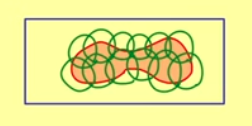
\includegraphics[width=0.3\textwidth]{Figs/compact_set.png}
    \caption{Compact set - every open cover has a finite subcover}
\end{figure}

We are already familiar with the Heine-Borel theorem for compact sets in \( \mathbb{R}^n \) with the standard topology.
\begin {theorem}{\textbf{Heine-Borel Theorem}} \\
    A subset \( A \subseteq \mathbb{R}^n \) is compact \( \Leftrightarrow A \) is closed and bounded.
\end{theorem}

We don't have this theorem for general topological spaces, simply because the term "bounded" is not defined in a general topological spaces.
If we had a metric we could define boundedness in terms of the metric, but even then the Heine-Borel theorem would not hold in general.

\begin{theorem}{\textbf{Compactness in hausdorff spaces}} \\
    Let \( (X, \mathcal{T}) \) be a hausdorff space and \( A \subseteq X \). \\ 
    If \( A \) is compact, then \( A \) is closed.
\end{theorem}

\begin{proof}
    Let \( A \) be a compact set in a hausdorff space \( X \). \\
    We want to show that \( A \) is closed. \\
    Let \( b \in X \setminus A \). 
    For every \( a \in A \), since \( X \) is hausdorff, there exist open sets \( U_a \) and \( V_a \) such that \( a \in U_a \), \( b \in V_a \), and \( U_a \cap V_a = \emptyset \). \\
    Then \( \{ U_a \}_{a \in A} \) is an open cover of \( A \). \\
    Since \( A \) is compact, there exists a finite subcover \( \{ U_{a_1}, U_{a_2}, \ldots, U_{a_n} \} \) of \( A \). \\
    Let \( V = \bigcap_{i=1}^n V_{a_i} \). \\
    Then \( V \) is an open set containing \( b \) and \( V \cap A = \emptyset \), which implies that \( b \) is an interior point of \( X \setminus A \). 
    Therefore, \( A \) is closed.
\end{proof}


% * * * * * * * * * * * * * * * * * * * * * * * *
% * * * * * * * * * * * * * * * * * * * * * * * *
% * * * * * * * * * * * * * * * * * * * * * * * *
% * * * * * * * * * * * * * * * * * * * * * * * *
% * * * * * * * * * * * * * * * * * * * * * * * *
% * * * * * * * * * * * * * * * * * * * * * * * *
% * * * * * * * * * * * * * * * * * * * * * * * *


\chapter{Locally Euclidean Spaces}

\begin{definition}{\textbf{n-dimensional (topological) Manifold}} \\
    A topological space \( (M , \mathcal{T}) \) is called a manifold of dimension \( n \) if it satisfies the following conditions:
    \begin{enumerate}
        \item \( (M , \mathcal{T}) \) is hausdorff space.
        \item \( (M , \mathcal{T}) \) is second countable.
        \item \( (M, \mathcal{T}) \) is locally euclidean of dimension \( n \).
    \end{enumerate}
\end{definition}

\begin{figure}[H]
    \centering
    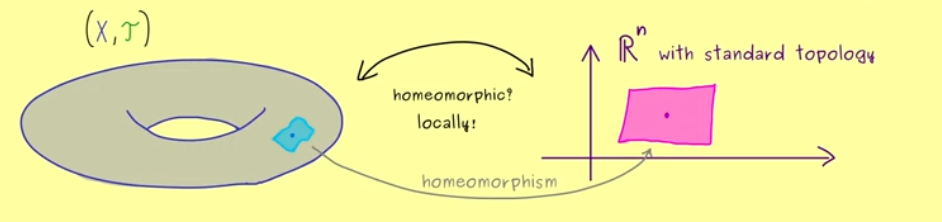
\includegraphics[width=\textwidth]{Figs/locally_euclidean_topological_space.png}
    \caption{Locally Euclidean Topological Space}
\end{figure}

\begin{definition}{\textbf{Locally Euclidean Space}} \\
    A topological space \( (M, \mathcal{T}) \) is locally euclidean of dimension \( n \) if \\ 
    \(\forall x \in M \), there exists an open neighborhood \( U \in \mathcal{T} \) and a homeomorphism \( h: U \to V \) where \( V \) is an open subset of \( \mathbb{R}^n \). \\
    Such an homeomorphism \( h: U \to V \) is called a \textbf{chart} of \( (M , \mathcal{T}) \) at \( x \).
\end{definition}

\begin{figure}[H]
    \centering
    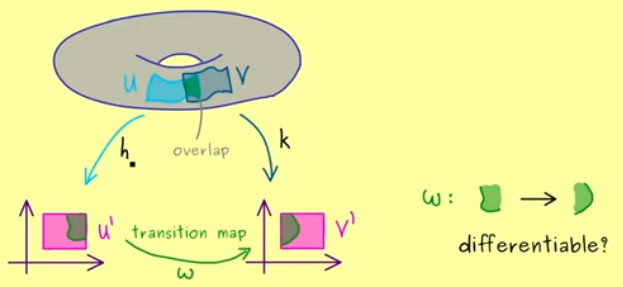
\includegraphics[width=0.7\textwidth]{Figs/chart_of_manifold.png}
    \caption{Charts and Atlases of a Manifold}
\end{figure}



% * * * * * * * * * * * * * * * * * * * * * * * *
% * * * * * * * * * * * * * * * * * * * * * * * *
% * * * * * * * * * * * * * * * * * * * * * * * *
% * * * * * * * * * * * * * * * * * * * * * * * *
% * * * * * * * * * * * * * * * * * * * * * * * *
% * * * * * * * * * * * * * * * * * * * * * * * *
% * * * * * * * * * * * * * * * * * * * * * * * *

\chapter{Examples of Manifolds}

\begin{definition}{\textbf{Atlas}} \\
    An atlas of a manifold \( M \) is a collection of charts that cover \( M \). \\
    Formally, an atlas \( \mathcal{A} \) of a manifold \( M \) is a collection of charts \( \{ (U_i, h_i) \}_{i \in I} \) such that 
    \begin{equation*}
        M = \bigcup_{i \in I} U_i
    \end{equation*}
\end{definition}

\begin{examples*} of Manifolds
    \begin{itemize}
        \item \( M , \mathcal{T} \) a discrete topological space with countably many points. \\
            Every point in \( M \) is a manifold of dimension 0.

        \item \( M \subseteq \mathbb{R}^n \) with the standard topology, \( (M , \mathcal{T}) \) is a manifold of dimension \( n \). \\
            h is the identity map and M is locally euclidean of dimension n (in fact, it is globally euclidean).

        \item \( S^2 = \{ x \in \mathbb{R}^3 : \| x \|_2 = 1 \} \) is a manifold of dimension 2. \\
            We have seen that \( S^2 \) is a hausdorff space. \\ 
            The atlas of \( S^2 \) consists of two charts: the upper hemisphere and the lower hemisphere. \\
            The upper hemisphere is the set \( U_{3, -} = \{ x \in S^2 : x_3 > 0 \} \) and the lower hemisphere is the set \( U_{3, -}^{'}= \{ x \in S^2 : x_3 < 0 \} \). \\
            The homeomorphism \( h_{3, -}: U_{3, -} \to \mathbb{R}^2 \) is defined as \( h_{3, -}(x_1, x_2, x_3) = (x_1, x_2) \). \\
            The inverse homeomorphism \( h_{3, -}^{-1}: \mathbb{R}^2 \to U_1 \) is defined as \( h_{3, -}^{-1}(x_1, x_2) = (x_1, x_2, \sqrt{1 - x_1^2 - x_2^2}) \). \\
            The same argument holds for the lower hemisphere. \\
            So \( (U_{i, \pm }, h_{i, \pm})_{i \in \{1,2,3\}} \) is an atlas of \( S^2 \).
    \end{itemize}
    
\end{examples*}


% * * * * * * * * * * * * * * * * * * * * * * * *
% * * * * * * * * * * * * * * * * * * * * * * * *
% * * * * * * * * * * * * * * * * * * * * * * * *
% * * * * * * * * * * * * * * * * * * * * * * * *
% * * * * * * * * * * * * * * * * * * * * * * * *
% * * * * * * * * * * * * * * * * * * * * * * * *
% * * * * * * * * * * * * * * * * * * * * * * * *

\chapter{Projective Space is a Manifold}

As we have seen that the sphere \( S^n = \{ x \in \mathbb{R}^{n+1} : \| x \|_2 = 1 \} \), 
is an n-dimensional manifold with atlas \( (U_{i, \pm}, h_{i, \pm})_{i \in \{1, \dots ,n+1\}} \) 
where \( U_{i, \pm} = \{ x \in \mathbb{R}^{n+1} : \pm x_i > 0 \} \) and \( h_{i, \pm}(x_1, \ldots, x_{n+1}) = (x_1, \ldots, x_{i-1}, x_{i+1}, \ldots, x_{n+1}) \).
We have also seen that the projective space \( \mathbf{P}^n (\mathbb{R}) = S^n / \sim \) with quotient topology and equivalence 
relation \( x \sim y \Leftrightarrow x = y \) or \( x = -y \). \\
We will show that the projective space \( \mathbf{P}^n (\mathbb{R}) \) is a manifold of dimension \( n \).

\medbreak

We will define \( V_i = \{ [x]_\sim \in \mathbf{P}^n : x_i \neq 0 \} \). 
Note that every equivilance class \( [x]_\sim \) contains exactly 2 points from the sphere \( S^n \).
\( q^{-1}[V_i] = U_{i, +} \cup U_{i, -} \) is an open set in the sphere \( S^n \) and \( q: S^n \to \mathbf{P}^n \) is a quotient map,
so \( V_i \) is an open set in the projective space \( \mathbf{P}^n \).

\medbreak

In order to show that \( \mathbf{P}^n (\mathbb{R}) \) is a manifold of dimension \( n \), 
we will present homeomorphisms \( h_i: V_i \to \mathbb{R}^n \) for each \( i \in \{1, \ldots, n+1\} \) such that \( (V_i, h_i) \) is a chart of \( \mathbf{P}^n (\mathbb{R}) \).

\begin{figure}[H]
    \begin{subfigure}{0.5\textwidth}
        \centering
        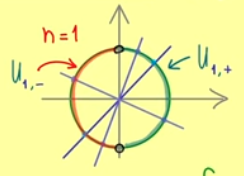
\includegraphics[width=0.5\textwidth]{Figs/projective_space_P1.png}
    \end{subfigure}
    \begin{subfigure}{0.5\textwidth}
        \centering
        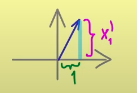
\includegraphics[width=0.5\textwidth]{Figs/projective_space_P1_2.png}
    \end{subfigure}
    \caption{Projective Space of dimension 1 as a quotient space of the circle}
\end{figure}

For n = 1: \\
\( V_1 = \{ [x]_\sim \in \mathbf{P}^1 : x_1 \neq 0 \} \) is an open set in \( \mathbf{P}^1 \). \\
\( q^{-1}[V_1] = U_{1, +} \cup U_{1, -} \) \\
We need homeomorphisms \( h_1: V_1 \to V_1' \) where \( V_1' \) is an open subset of \( \mathbb{R} \). \\
We can define \( h_1: V_1 \to V_1' \) as \( h_1([x]_\sim) = \frac{x_2}{x_1} \) (the slope) for \( x_1 \neq 0 \). \\
The invese homeomorphism \( h_1^{-1}: V_1' \to V_1 \) is defined as \( h_1^{-1}(x1) = [ \binom{1}{x1'} \cdot \frac{1}{\sqrt{1^2 + ({x1'})^2}} ]_\sim \). \\
\( V_2 = \{ [x]_\sim \in \mathbf{P}^1 : x_2 \neq 0 \} \) and we will do the same with the change of coordinates.

\medbreak

For $n \in \mathbb{N}$: \\
\( V_i = \{ [x]_\sim \in \mathbf{P}^n : x_i \neq 0 \} \) is an open set in \( \mathbf{P}^n \). \\
\( q^{-1}[V_i] = U_{i, +} \cup U_{i, -} \) \\
We need homeomorphisms \( h_i: V_i \to V_i' \) where \( V_i' \) is an open subset of \( \mathbb{R}^n \). \\
We can define \( h_i: V_i \to V_i' \) as \( h_i([x]_\sim) = \frac{1}{x_i} (x_1, \ldots, x_{i-1}, x_{i+1}, \ldots, x_{n+1}) \) for \( x_i \neq 0 \). \\
In the inverse we apply 1 to the i-th coordinate and normalize the vector.



% * * * * * * * * * * * * * * * * * * * * * * * *
% * * * * * * * * * * * * * * * * * * * * * * * *
% * * * * * * * * * * * * * * * * * * * * * * * *
% * * * * * * * * * * * * * * * * * * * * * * * *
% * * * * * * * * * * * * * * * * * * * * * * * *
% * * * * * * * * * * * * * * * * * * * * * * * *
% * * * * * * * * * * * * * * * * * * * * * * * *

\chapter{Smooth structures (differential structures)}

\begin{definition}{\textbf{Transition map}} \\
    Let \( (M, \mathcal{T}) \) be an n-manifold and \( (U, h) \) and \( (V, k) \) be two charts of \( M \). \\
    The transition map \( \omega : h(U \cap V) \to k(U \cap V) \) is called the transition map between the charts \( (U, h) \) and \( (V, k) \).
\end{definition}

Note that the transition map is a transoformation of subset of the $R^n$ space, it does not have to be a linear transformation.

We have seen in definition~\ref{def:C^2_class} that a function \( f: \mathbb{R}^n \to \mathbb{R} \) is of class \( C^2 \) 
if all partial derivatives of \( f \) up to order 2 exist and are continuous. We can extend this definition to manifolds.

\begin{definition}{\textbf{$C^k$-Diffeomorphism (Vector Space)}} \\
    A function \( \omega : \mathbb{R}^n \to \mathbb{R}^n \) $C^k$-diffeomorphism ($ k \in \{0, 1, \cdots\} \cup \{ \infty \} $) if the following conditions hold:
    \begin{enumerate}
        \item \( \omega \) is k times continuously differentiable (partial derivatives up to order k exist and are continuous).
        \item \( \omega \) is bijective (both injective and surjective - one-to-one and onto).
        \item The inverse function \( \omega^{-1} \in C^k \).
    \end{enumerate}
\end{definition}

If $k = \infty$, then \( \omega \) is called a smooth diffeomorphism (or simply a diffeomorphism) - all partial derivatives of \( \omega \) exist and are continuous. \\
If $k = 0$, then \( \omega \) is called a homeomorphism - \( \omega \) is continuous, bijactive, 
and the inverse function \( \omega^{-1} \) is continuous (see definition~\ref{def:homeomorphism}). By the composition of charts, the transition map is a always a homeomorphism.

\begin{definition}{\textbf{$C^k$-smoothly compatible charts}} \\
    Two charts \( (U, h) \) and \( (V, k) \) of a manifold \( M \) are called \( C^k \)-smoothly compatible 
    if the transition map \( \omega: h(U \cap V) \to k(U \cap V) \) is a \( C^k \)-diffeomorphism.
\end{definition}

(If $k = \infty$, then the charts are called smoothly compatible.)

What happens if any two charts of a manifold are $C^k$-smoothly compatible?

\begin{definition}{\textbf{$C^k$-atlas}} \\
    An atlas \( \mathcal{A} = \{ (U_i, h_i) \}_{i \in I} \) of a manifold \( M \) is called a \( C^k \)-atlas 
    if every pair of charts in \( \mathcal{A} \) are \( C^k \)-smoothly compatible.
\end{definition}


\begin{definition}{\textbf{Maximal $C^k$-atlas ($C^k$-smooth structure)}} \\
    A maximal \( C^k \)-atlas of a manifold \( M \) is \( \mathcal{A} \) is:
    \begin{enumerate}
        \item \( \mathcal{A} \) is a \( C^k \)-atlas of \( M \).
        \item For any other \( C^k \)-atlas \( \mathcal{B} \) of \( M \), \( \mathcal{A} \nsubseteq \mathcal{B} \).
    \end{enumerate}
\end{definition}


\begin{definition}{\textbf{n-dimensional $C^k$-smooth manifold}} \\
    A manifold \( M \) is called a \( C^k \)-smooth manifold if: 
    \begin{enumerate}
        \item \( M \) is n-dimensional topological manifold.
        \item There exists a maximal \( C^k \)-atlas of \( M \).
    \end{enumerate}
\end{definition}




% * * * * * * * * * * * * * * * * * * * * * * * *
% * * * * * * * * * * * * * * * * * * * * * * * *
% * * * * * * * * * * * * * * * * * * * * * * * *
% * * * * * * * * * * * * * * * * * * * * * * * *
% * * * * * * * * * * * * * * * * * * * * * * * *
% * * * * * * * * * * * * * * * * * * * * * * * *
% * * * * * * * * * * * * * * * * * * * * * * * *

\chapter{Examples of smooth manifolds}

\begin{example*}{\textbf{The n-dimensional Euclidean sphere \( S^n \subseteq \mathbb{R}^{n+1} \)}} \\
    We have seen that the sphere \( S^n = \{ x \in \mathbb{R}^{n+1} : \| x \|_2 = 1 \} \), 
    is an n-dimensional manifold with atlas \( (U_{i, \pm}, h_{i, \pm})_{i \in \{1, \dots ,n+1\}} \) 
    where \( U_{i, \pm} = \{ x \in \mathbb{R}^{n+1} : \pm x_i > 0 \} \) and \( h_{i, \pm}(x_1, \ldots, x_{n+1}) = (x_1, \ldots, x_{i-1}, x_{i+1}, \ldots, x_{n+1}) \).
    
    \begin{figure}[H]
        \centering
        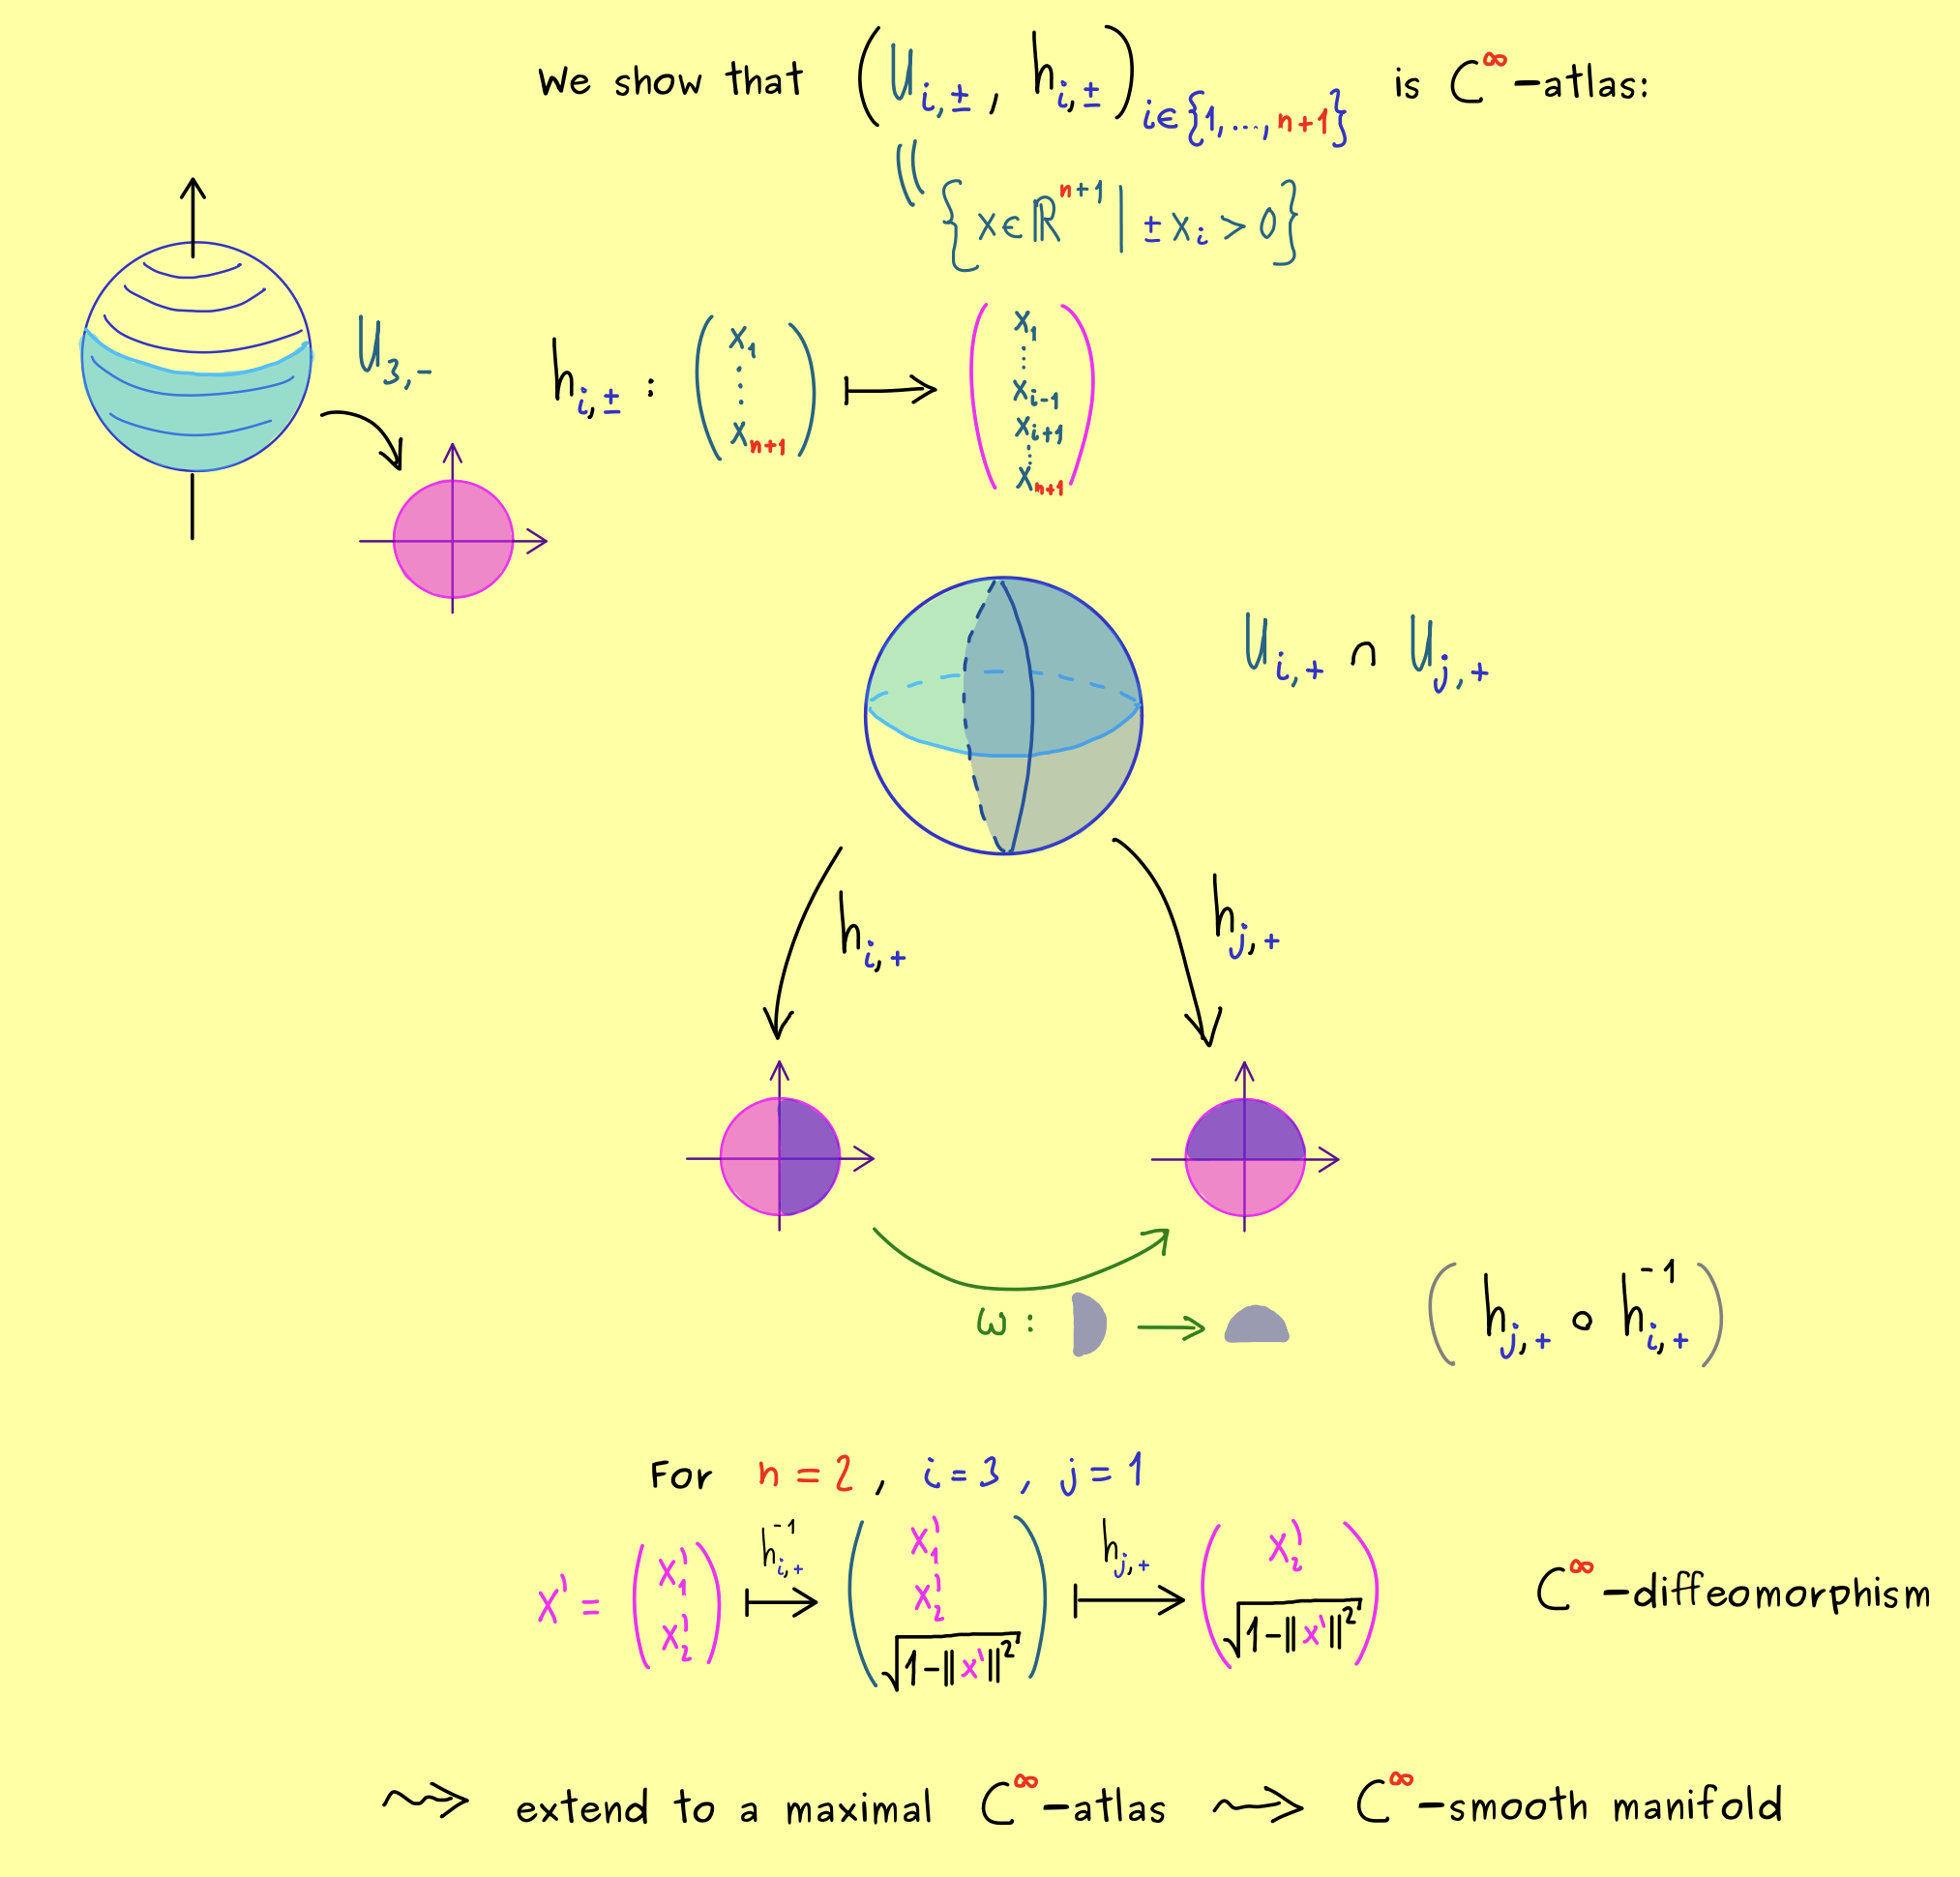
\includegraphics[width=\textwidth]{Figs/sphere_is_C^k_smooth.png}
        \caption{Sphere \( S^n \) is an n-dimensional $C^{\infty}$ smooth manifold}
    \end{figure}
    
\end{example*}

\begin{example*}{\textbf{$\mathbb{R}^n$ is a $C^{\infty}$ smooth manifold}} \\
    The Euclidean space \( \mathbb{R}^n \) is a \( C^{\infty} \) smooth manifold with the atlas \( \{ (\mathbb{R}^n, id) \} \).
    The is the standard smooth structure of \( \mathbb{R}^n \).
\end{example*}

\begin{example*}{\textbf{Consider $f \in C^1$}} \\
    Let \( f: \mathbb{R} \to \mathbb{R} \) be a function of class \( C^1 \). \\
    Let $ G_f = \{ (x, f(x)) \in \mathbb{R}^2 : x \in \mathbb{R} \} $ be the graph of \( f \). \\
    Then \( G_f \) is a \( C^1 \) smooth manifold with one chart: \( h : G_f \to \mathbb{R} \) defined as \( h(x, f(x)) = x \).
\end{example*}

In fact any graph of a function of class \( C^k \) is a \( C^k \) smooth manifold.
We can also observe that $G_f$ is a 1-dimensional $C^1$-smooth manifold that is embedded in another smooth manifold, \( \mathbb{R}^2 \).

% * * * * * * * * * * * * * * * * * * * * * * * *
% * * * * * * * * * * * * * * * * * * * * * * * *
% * * * * * * * * * * * * * * * * * * * * * * * *
% * * * * * * * * * * * * * * * * * * * * * * * *
% * * * * * * * * * * * * * * * * * * * * * * * *
% * * * * * * * * * * * * * * * * * * * * * * * *
% * * * * * * * * * * * * * * * * * * * * * * * *

\chapter{Submanifolds}

\begin{definition}{\textbf{Submanifold}} \\
    Let \( M \) be a an n-dimensional smooth manifold. 
    \( M_0 \subseteq M \) is called a k-dimensional submanifold of \( M \) if for every \( p \in M_0 \), there exists a chart \( (U, h) \) of \( M \) 
    such that \( h(U \cap M_0) = h(U) \cap (\mathbb{R}^k \times \{ 0 \}^{n-k}) \).
    \((U, h)\) is called a \textbf{submanifold chart} for \( M_0 \).
\end{definition}

Note: \( M_0 \) is also a manifold: 
\( (U, h) submanifold chart \to (\hat{U}, \hat{h}) \) chart, \( \hat{U} = U \cap M_0 \), \( \hat{h} = h|_{\hat{U}} \).

% * * * * * * * * * * * * * * * * * * * * * * * *
% * * * * * * * * * * * * * * * * * * * * * * * *
% * * * * * * * * * * * * * * * * * * * * * * * *
% * * * * * * * * * * * * * * * * * * * * * * * *
% * * * * * * * * * * * * * * * * * * * * * * * *
% * * * * * * * * * * * * * * * * * * * * * * * *
% * * * * * * * * * * * * * * * * * * * * * * * *

\chapter{Regular value theorem in \( \mathbb{R}^n \)}

\begin{definition}{\textbf{Critical point}} \\
    Let \( f: U \to \mathbb{R}^m \), \( U \subseteq \mathbb{R}^n \) open, \( C^1 \)-function. \\
    A point \( x \in U \) is called a critical point of f if the Jacobian matrix of f at x has rank less than m.
\end{definition}

\begin{definition}{\textbf{Regular value}} \\
    Let \( f: U \to \mathbb{R}^m \), \( U \subseteq \mathbb{R}^n \) open, \( C^1 \)-function. \\
    A point \( y \in f[U] \) is called a regular value of f if for every \( x \in f^{-1}(y) \), x is not a critical point of f.
\end{definition}

\begin{theorem}{\textbf{Regular value theorem in \( \mathbb{R}^n \)}} \\
    Let \( f: U \to \mathbb{R}^m \), \( U \subseteq \mathbb{R}^n \) open, \( C^\infty \)-function. \\
    If c is a regular value of f, then \( f^{-1}[\{c\}] \) is a submanifold of \( \mathbb{R}^n \) of dimension \( n - m \).
\end{theorem}

For example if \( f: \mathbb{R}^n \to \mathbb{R} \), \( f(x_1, \dots, x_n) = x_1^2 + \dots + x_n^2 \), then 0 is a regular value of f. \\
let \( 0 \neq r \in \mathbb{R} \), then r is a regular value of f, for example \( r = 1 \).
Then the sphere \( S^{n-1} \) is a submanifold of \( \mathbb{R}^n \) of dimension \( n - 1 \).


% * * * * * * * * * * * * * * * * * * * * * * * *
% * * * * * * * * * * * * * * * * * * * * * * * *
% * * * * * * * * * * * * * * * * * * * * * * * *
% * * * * * * * * * * * * * * * * * * * * * * * *
% * * * * * * * * * * * * * * * * * * * * * * * *
% * * * * * * * * * * * * * * * * * * * * * * * *
% * * * * * * * * * * * * * * * * * * * * * * * *

\chapter{Smooth maps}

Until now we have defined smooth manifolds (and \( C^k \)-smooth manifolds). \\
Recall that 
\begin{itemize}
    \item an n-dimensional manifold is a topological space that is locally euclidean of dimension n and hausdorff and second countable.
    \item a smooth manifold is a topological manifold with a maximal \( C^{\infty} \)-atlas.
    \item a \( C^{\infty} \)-atlas is a collection of charts that cover the manifold and the transition 
    maps between any two charts are \( C^{\infty} \)-diffeomorphisms.
    \item \( C^k \)-diffeomorphism is a function that is k times continuously differentiable, bijective, and the inverse function is also \( C^k \).
\end{itemize}

\begin{figure}
    \centering
    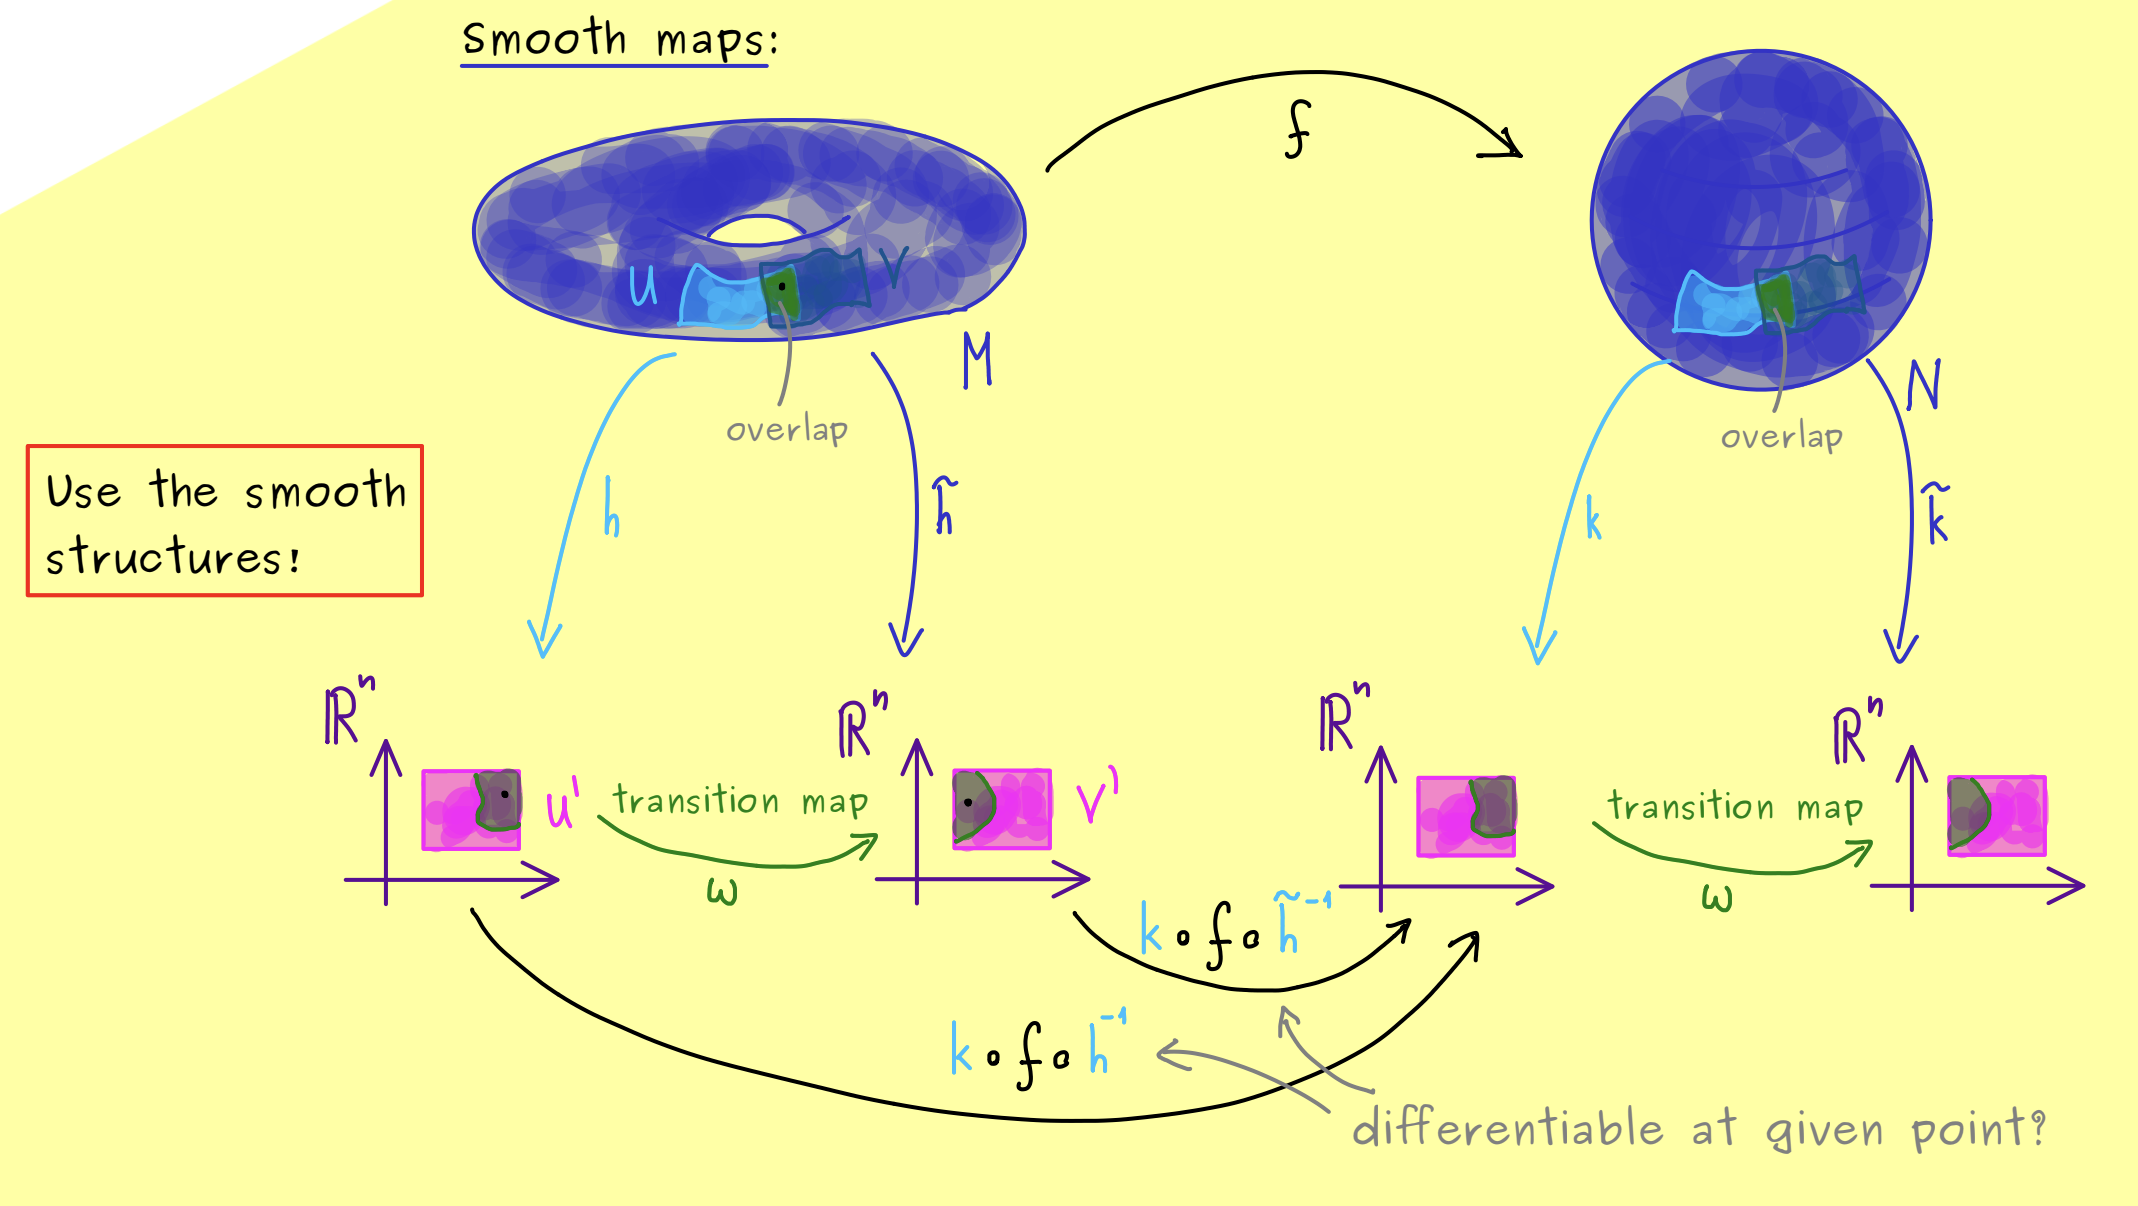
\includegraphics[width=\textwidth]{Figs/smooth_maps.png}
    \caption{Smooth map between two manifolds}
\end{figure}

\begin{definition}{\textbf{k-times differentiable map at a point}} \\
    Let \( f: M \to N \) be a map between two smooth manifolds. \\
    f is called k-times differentiable at a point \( p \in M \) if for every chart \( (U, h) \) of M and every chart \( (W, k) \) of N, 
    with \( p \in U \) and \( f(p) \in V \), the map \( k \circ f \circ h^{-1} \) is k-times differentiable at \( h(p) \).
\end{definition}

\begin{definition}{\textbf{(\(C^\infty\)) Smooth map}} \\
    Let \( f: M \to N \) be a map between two smooth manifolds. \\
    f is called smooth if f is k-times differentiable at every point \( p \in M \) for every \( k \in \mathbb{N} \).
\end{definition}

We often denote the set of smooth maps between two smooth manifolds M and N as \( C^\infty(M, N) \).

% * * * * * * * * * * * * * * * * * * * * * * * *
% * * * * * * * * * * * * * * * * * * * * * * * *
% * * * * * * * * * * * * * * * * * * * * * * * *
% * * * * * * * * * * * * * * * * * * * * * * * *
% * * * * * * * * * * * * * * * * * * * * * * * *
% * * * * * * * * * * * * * * * * * * * * * * * *
% * * * * * * * * * * * * * * * * * * * * * * * *

\chapter{Examples of smooth maps}

\begin{itemize}
    \item \( S^2 \rightarrow \mathbb{R}^3\) where i is the identity matrix.
    \item the quotient map \( q : S^2 \rightarrow P^2(\mathbb{R}) = S^2 / \sim \)
\end{itemize}


% * * * * * * * * * * * * * * * * * * * * * * * *
% * * * * * * * * * * * * * * * * * * * * * * * *
% * * * * * * * * * * * * * * * * * * * * * * * *
% * * * * * * * * * * * * * * * * * * * * * * * *
% * * * * * * * * * * * * * * * * * * * * * * * *
% * * * * * * * * * * * * * * * * * * * * * * * *
% * * * * * * * * * * * * * * * * * * * * * * * *

\chapter{Regular value theorem (abstract version)}

\begin{definition}{\textbf{Critical point}} \\
    Let \( f: M \to N \) be a smooth map between two smooth manifolds of dimensions m and n ($m \geq n$). \\
    Let \( p \in M \), \( (U, h) \) a chart of M at p and \((V, k)\) be a chart of N at \(f(p)\). \\
    A point \( p \in M \) is called a critical point of f if 
    \begin{equation*}
        rank(f_p) := rank(J_{k \circ f \circ h^{-1}}(h(p))) < n
    \end{equation*}
\end{definition}
    

\begin{theorem}{\textbf{Regular value theorem (abstract version)}} \\
    Let \( f: M \to N \) be a smooth map between two smooth manifolds of dimensions n and m ($m \geq n$).
    Let \( q \in N \) be a regular value of f. \\
    Then \( f^{-1}[\{q\}] \) is a submanifold of M of dimension \( m - n \).
\end{theorem}

% * * * * * * * * * * * * * * * * * * * * * * * *
% * * * * * * * * * * * * * * * * * * * * * * * *
% * * * * * * * * * * * * * * * * * * * * * * * *
% * * * * * * * * * * * * * * * * * * * * * * * *
% * * * * * * * * * * * * * * * * * * * * * * * *
% * * * * * * * * * * * * * * * * * * * * * * * *
% * * * * * * * * * * * * * * * * * * * * * * * *

\chapter{Tangent space for submanifolds}

\begin{definition}{\textbf{Local parametrization of a submanifold}} \\
    Let \( M \) be an n-dimensional smooth manifold and \( M_0 \subseteq M \) be a k-dimensional submanifold of \( M \). \\
    Let \( p \in M_0 \) and \( (U, h) \) be a submanifold chart for \( M_0 \) at p, where \( h: U \to U', \quad U' \subseteq \mathbb{R}^k \) is a homeomorphism. \\
    The function \( \varphi : \mathbb{R}^k \cap U' \to M \cap U \) is called a local parametrization of \( M_0 \) at p.
\end{definition}

\begin{example*}The circle
    Let \( S^1 = \{ x \in \mathbb{R}^2 : \| x \|_2 = 1 \} \) be the unit circle in \( \mathbb{R}^2 \). \\
    Let \( M_0 = \{ x \in S^1 : x_1 > 0 \} \) be the right half of the circle. \\
    Let \( p = (1, 0) \in M_0 \) and \( (U, h) \) be a submanifold chart for \( M_0 \) at p, where \( h: U \to U' \) is a homeomorphism. \\
    The function \( \varphi : (0, 2\pi) \to M \cap U \) defined as \( \varphi(t) = (\cos(t), \sin(t)) \) is a local parametrization of \( M_0 \) at p.    
\end{example*}

\begin{definition}{\textbf{The Tangent Space of a submanifold}} \\
    Let \( (M \subseteq \mathbb{R}^n) \) be a k-dimensional submanifold of \( \mathbb{R}^n \). \\
    Let \( p \in M \) and \( \varphi : U' \to U \) be a local parametrization of \( M \) at p. \\
    Let \( \tilde{p} = \varphi^{-1}(p) \). \\
    The tangent space of \( M \) at p is defined as 
    \begin{equation*}
        T_p^{sub} M = d\varphi_{\tilde{p}}[\mathbb{R}^k] = \{ J_{\varphi}(\varphi^{-1}(p)) \cdot v : v \in \mathbb{R}^k \}
    \end{equation*}
\end{definition}

Note thet \( T_p^{sub} M \subseteq \mathbb{R}^n \) is a k-dimensional subspace.
If \( M = \mathbb{R}^n \), then $\phi = \phi^{-1}=id$ , $J_{\phi}(\phi^{-1}(p)) = I$ and $T_p^{sub} \mathbb{R}^n = \mathbb{R}^n$.


% * * * * * * * * * * * * * * * * * * * * * * * *
% * * * * * * * * * * * * * * * * * * * * * * * *
% * * * * * * * * * * * * * * * * * * * * * * * *
% * * * * * * * * * * * * * * * * * * * * * * * *
% * * * * * * * * * * * * * * * * * * * * * * * *
% * * * * * * * * * * * * * * * * * * * * * * * *
% * * * * * * * * * * * * * * * * * * * * * * * *

\chapter{Tangent curves}

\begin{definition}{\textbf{Smooth curve}} \\
    Let \( M \) be an n-dimensional smooth manifold. \\
    A smooth curve in M is a smooth map \( \gamma: I \to M \) where I is an open interval in \( \mathbb{R} \).
\end{definition}


\begin{definition}{\textbf{Differentiable curve on a manifold \( M \)}} \\
    A differentiable curve on a manifold \( M \) is a function \( \gamma: I \to M \), where \( I \) is an interval in \( \mathbb{R} \). 
    The curve \( \gamma \) is differentiable at a point \( t_0 \in I \) if for every chart 
    \( (U, \phi) \) of \( M \) with \( \gamma(t_0) \in U \), the composition \( \phi \circ \gamma: I \to \mathbb{R}^n \) is differentiable at \( t_0 \). 
    A curve is said to be differentiable on \( I \) if it is differentiable at every point in \( I \).
\end{definition}

\begin{definition}{\textbf{Tangent curve}} \\
    Let \( M \) be an n-dimensional smooth manifold and \( \gamma: I \to M \) be a smooth curve in M. \\
    Let \( p = \gamma(t_0) \) for some \( t_0 \in I \). \\
    The tangent curve of \( \gamma \) at \( t_0 \) is defined as 
    \begin{equation*}
        \gamma'(t_0) = d\gamma_{t_0}[\mathbb{R}]
    \end{equation*}
\end{definition}

The derivative \( \gamma'(t_0) \) at \( t_0 \) is then defined to be a vector in the tangent space \( T_{\gamma(t_0)}M \).


\begin{definition}{\textbf{The Tangent Space of a submanifold}} \\
    Let \( M \subseteq \mathbb{R}^n \) be a k dimensional submanifold and \( p \in M \). 
    The tangent space of \( M \) at \( p \) is:
    \begin{equation*}
        T_p^{sub}M = \{ \gamma'(0) \quad | \quad \gamma : (-\epsilon, \epsilon) \to M \quad \text{differentiable and} \quad \gamma(0) = p \}        
    \end{equation*}
\end{definition}


\begin{theorem}{\textbf{The 2 definitions for the tangent space of submanifold are equivalent}} \\
    Let \( M \subseteq \mathbb{R}^n \) be a k-dimensional submanifold and \( p \in M \). \\
    Let \( \varphi : U' \to U \) be a local parametrization of \( M \) at \( p \). \\
    Let \( \tilde{p} = \varphi^{-1}(p) \). Then 
    \begin{equation*}
        T_p^{sub}M = \{ J_{\varphi}(\varphi^{-1}(p)) \cdot x : x \in \mathbb{R}^k \} = 
        \{ \gamma'(0) \quad | \quad \gamma : (-\epsilon, \epsilon) \to M \quad \text{differentiable and} \quad \gamma(0) = p \}
    \end{equation*}    
\end{theorem}

\begin{proof}{We will show double inclusion between the groups:} \\

    Let \( \gamma : (-\epsilon, \epsilon) \to M \) be a smooth curve in M with \( \tilde{\gamma}(0) = p \). \\
    Let \( \tilde{\gamma} : (-\epsilon, \epsilon) \to U' \subseteq \mathbb{R}^k \) be the curve defined as \( \tilde{\gamma}(t) = \varphi^{-1}(\gamma(t)) \). \\
    
    \( \subseteq \): \( v \in \{ J_{\varphi}(\varphi^{-1}(p)) \cdot x : x \in \mathbb{R}^k \} \) \\
    \( v = J_{\varphi}(\tilde{\gamma}(0)) \cdot \tilde{\gamma}'(0) \)  with \( \tilde{\gamma}(t) = \tilde{p} + t( \tilde{\gamma}'(0)) \) \\ 
    Then \( v = \frac{d}{dt}(\varphi \circ \tilde{\gamma}) \mid _{t=0} = \frac{d}{dt}(\gamma) \mid _{t=0} = \gamma'(0) \) \\

    \medbreak
    \( \supseteq \): \( v \in \{ \gamma'(0) \quad | \quad \gamma : (-\epsilon, \epsilon) \to M \quad \text{differentiable and} \quad \gamma(0) = p \} \) \\
    There exists an open set \( U \) such that \( \forall y \in (-\epsilon, \epsilon)\quad \gamma(y) \in U \). \\
    Let \( \tilde{\gamma} : (-\epsilon, \epsilon) \to U' \) be defined as \( \tilde{\gamma}(t) = \varphi^{-1}(\gamma(t)) \). \\
    Then \( \tilde{\gamma}'(0) = \frac{d}{dt}(\varphi^{-1} \circ \gamma) \mid _{t=0} = J_{\varphi}^{-1}(\gamma(0)) \cdot \gamma'(0) \in T_p^{sub}M \)  
\end{proof}



% * * * * * * * * * * * * * * * * * * * * * * * *
% * * * * * * * * * * * * * * * * * * * * * * * *
% * * * * * * * * * * * * * * * * * * * * * * * *
% * * * * * * * * * * * * * * * * * * * * * * * *
% * * * * * * * * * * * * * * * * * * * * * * * *
% * * * * * * * * * * * * * * * * * * * * * * * *
% * * * * * * * * * * * * * * * * * * * * * * * *

\chapter{Tangent space (definition via tangent curves)}

Now we will define the tangent space of an abstract smooth manifold (that is not embedded in \( \mathbb{R}^n \)).

\begin{definition}{\textbf{The set of smooth curves that pass throught p  $(C_p(M))$}} \\
    Let \( M \) be an k-dimensional smooth manifold and \( p \in M \). \\
    \begin{equation*}
        C_p(M) = \{ \gamma : (-\epsilon, \epsilon) \to M \quad | \quad \gamma \quad \text{differentiable and} \quad \gamma(0) = p \} 
    \end{equation*}
\end{definition}

Let \( \gamma , \alpha \) be two smooth curves in \( C_p(M) \) and \( (U, h) \) be a chart of \( M \) at \( p \). \\
We define the equivalence relation $ \gamma \sim \alpha \iff  (h \circ \gamma )'(0) = (h \circ \alpha)'(0) $. \\ 
The equivalence classes of \( C_p(M) \) are denoted as \( [ \gamma ]_\sim \) and each equivalence class repsents a tangent vector at \( p \). \\

\begin{definition}{\textbf{Tangent space of a smooth manifold}} \\
    Let \( M \) be an k-dimensional smooth manifold and \( p \in M \). \\
    The tangent space of \( M \) at \( p \) is defined as 
    \begin{equation*}
        T_pM = C_p(M)/\sim \quad = \{ [ \gamma ]_\sim \quad | \quad \gamma \in C_p(M) \}
    \end{equation*}
\end{definition}

Result: 
\begin{itemize}
    \item For a submanifold \( M \subseteq \mathbb{R}^n \), \( T_p^{sub}M = T_pM \quad (\gamma'(0) \iff [\gamma]_\sim) \).
    \item Let \( v, w \in T_pM \text{ and } \lambda \in \mathbb{R} \). Then \(T_pM\) is a vector space with the operations: 
        \begin{itemize}
            \item \( v + w := h_*(v) + h_*(w) \) with \( h_* : [ \gamma ]_\sim \to (h \circ \gamma )'(0) \) \\
            ($h_*$ sends an equivalence class of curves to their common tangent vector in \( \mathbb{R}^k \)).
            \item \( \lambda \cdot v := h_*^{-1} (\lambda \cdot h_*(v)) \)
        \end{itemize}
\end{itemize}


% * * * * * * * * * * * * * * * * * * * * * * * *
% * * * * * * * * * * * * * * * * * * * * * * * *
% * * * * * * * * * * * * * * * * * * * * * * * *
% * * * * * * * * * * * * * * * * * * * * * * * *
% * * * * * * * * * * * * * * * * * * * * * * * *
% * * * * * * * * * * * * * * * * * * * * * * * *
% * * * * * * * * * * * * * * * * * * * * * * * *

\chapter{Coordinate bases}


Let \( M \) be an n-dimensional smooth manifold and \( (U, h) \) be a chart of \( M \) at \( p \). \\
Then $h$ is a homeomorphism between \( U \) and an open set \( U' \subseteq \mathbb{R}^n \). \\
Let \(\varphi = h^{-1} : U' \to U \) be the inverse of \( h \) (it exists and smooth (homeomorphism) by definition). \\
Let \( \tilde{p} = h(p) \). We have seen that the tangent space of \( M \) at \( p \) is \( T_pM = C_p(M)/\sim \). \\
The tangent space \( T_pM \) can also be mapped to \( \mathbb{R}^n \) by the map \( h_* : T_pM \to \mathbb{R}^n \) defined as
\begin{equation*}
    h_*([ \gamma ]_\sim) = (h \circ \gamma)'(0) 
\end{equation*}
In fact, as n is the dimension of \( M \), n is also the dimension of \( T_pM \) that means $h_*$ is linear and bijective $\Rightarrow h_*$ is an isomorphism.

\begin{definition}{\textbf{Coordinate basis (standard basis with respect to $(U, h)$)}} \\
    For $(U, h)$ and $ p \in U$ we define the tangent vector $\partial_j := \varphi_*(e_j)$ where $(e_1, \ldots, e_n)$ is the standard basis of $\mathbb{R}^n$.
    The set $\{ \partial_1, \ldots, \partial_n \}$ is called the coordinate basis of $T_pM$ with respect to $(U, h)$.
\end{definition}

Remark: For n-dimensional submanifolds $M \subseteq \mathbb{R}^N$, $T_p^{sub}M = T_pM \cong \mathbb{R}^n$ and $\varphi_*(e_j) = J_{\varphi}(\tilde{p}) \cdot e_j$,
and $(\partial_1, \ldots, \partial_n)$ is essentially $(\frac{\partial \varphi}{\partial x_1}(\tilde{p}), \ldots, \frac{\partial \varphi}{\partial x_n}(\tilde{p}))$.

We have already defined what a smooth map $f : M \to N$ is, \\
next we will define the differential of a smooth map $df_p : T_pM \to T_pN$.


% * * * * * * * * * * * * * * * * * * * * * * * *
% * * * * * * * * * * * * * * * * * * * * * * * *
% * * * * * * * * * * * * * * * * * * * * * * * *
% * * * * * * * * * * * * * * * * * * * * * * * *
% * * * * * * * * * * * * * * * * * * * * * * * *
% * * * * * * * * * * * * * * * * * * * * * * * *
% * * * * * * * * * * * * * * * * * * * * * * * *

\chapter{Differential (definition)}

\begin{definition}{\textbf{Tangent Bandle}} \\
    Let \( M \) be an n-dimensional smooth manifold and \( p \in M \). \\
    The tangent bandle of \( M \) is defined as
    \begin{equation*}
        TM := \sqcup _{p \in M} T_pM := \cup_{p \in M} \{ p \} \times T_pM
    \end{equation*}
\end{definition}

Note:
\begin{itemize}
    \item  $\sqcup$ is the disjoint union.
    \item Note that if \( M \) is a submanifold of \( \mathbb{R}^n \), then the union of the tangent spaces of \( M \) is not necessarily disjoint.
    \item The tangent bandle \( TM \) is a smooth manifold of dimension \( 2n \).
\end{itemize}

Recall, a map \( f: M \to N \) is called $C^k$-smooth if 
\begin{align*}
    &\forall p \in M, \quad \exists \text{ a chart } (U, h) \text{ of } M \text{ at } p \text{ and a chart } (V, k) \text{ of } N \text{ at } f(p) \text{ such that } \\
    &k \circ f \circ h^{-1} \text{ is } k \text{ times differentiable at } h(p).
\end{align*}
For each point $p \in M$, we define the differential of $f$ at $p$ as a linear map $df_p : T_pM \to T_{f(p)}N$, denoted as $df_p([\gamma])$ for $[\gamma] \in T_pM$.

\begin{figure}[H]
    \centering
    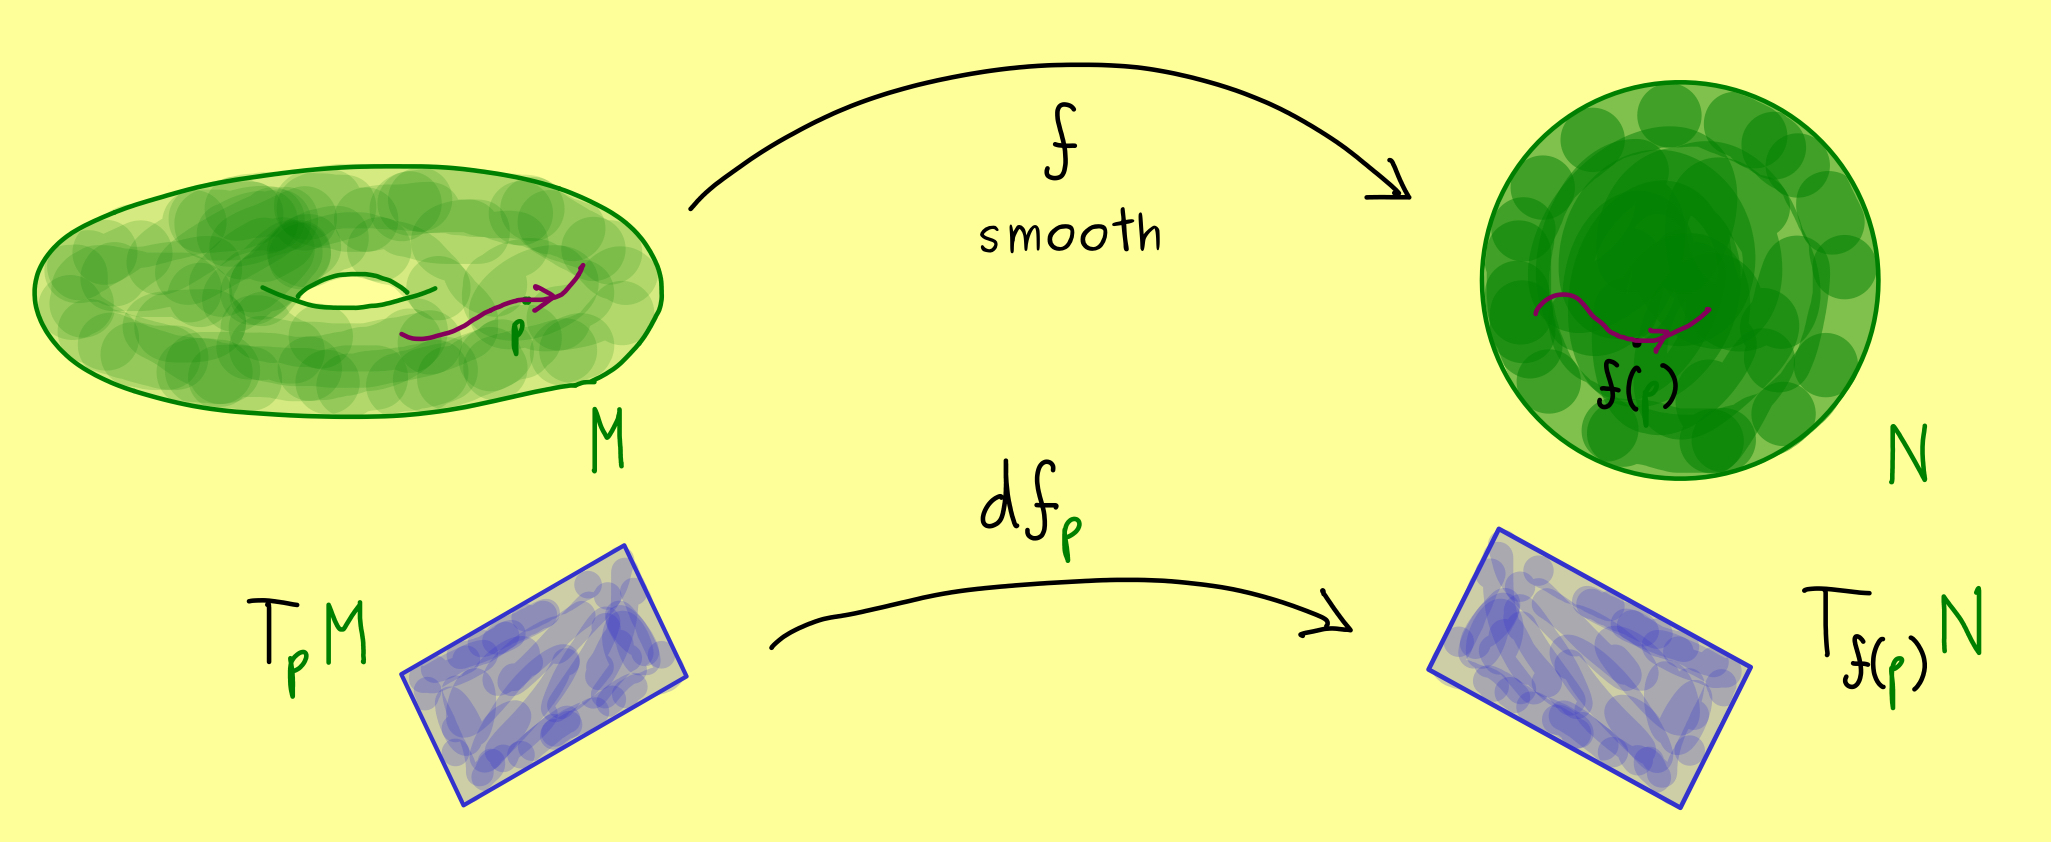
\includegraphics[width=0.7\textwidth]{Figs/differential_of_a_map_between_manifolds.jpeg}
    \caption{Differential of a smooth map}
\end{figure}

\begin{definition}{\textbf{Differential of f at point p}} \\
    Let \( f: M \to N \) be a smooth map between two smooth manifolds. \\
    Let \( p \in M \) and \( [\gamma] \in T_pM \). The differential of \( f \) at \( p \) is defined as \\
    \begin{equation*}
        df_p([\gamma]) = [f \circ \gamma] \in T_{f(p)}N
    \end{equation*}
\end{definition}

The linear map given by the differential is a linear approximation of the map \( f \) at the point \( p \). 

\begin{definition}{\textbf{Differential}} \\
    \begin{equation*}
        df : M \to TN \quad \text{defined as} \quad df(p) = df_p
    \end{equation*}
\end{definition}

\bigbreak

Example for submanifolds: \\
Let \( M , N \) be submanifolds of \( \mathbb{R}^n \), $p \in M$ and \( f: M \to N \) be a smooth map. \\
In this case, \(T_{f(p)}N = T_{f(p)}^{sub}N \). \\
$df_p ([\gamma]_{\sim}) = [f \circ \gamma_p]_{\sim} \stackrel{\text{bijection}}{=} (f \circ \gamma_p)'(0)$

\bigbreak

Example for $f : \mathbb{R}^n \to \mathbb{R}$ a smooth map: \\
$df_p([\gamma]_{\sim}) = (f \circ \gamma)'(0) = J_f(\gamma(0)) \cdot \gamma'(0) = \nabla f(p) \cdot \gamma'(0)$ \\
and we get that it's exactly the directional derivative of $f$ at $p$ along $[\gamma]$.

% * * * * * * * * * * * * * * * * * * * * * * * *
% * * * * * * * * * * * * * * * * * * * * * * * *
% * * * * * * * * * * * * * * * * * * * * * * * *
% * * * * * * * * * * * * * * * * * * * * * * * *
% * * * * * * * * * * * * * * * * * * * * * * * *
% * * * * * * * * * * * * * * * * * * * * * * * *
% * * * * * * * * * * * * * * * * * * * * * * * *

\chapter{Differential in Local charts}

Let \( f: M \to N \) be a smooth map from n-dimensional smooth manifold \( M \) to m-dimensional smooth manifold \( N \). \\
Let $p \in M$ and $(U, h)$ be a chart of $M$ at $p$ and $(V, k)$ be a chart of $N$ at $f(p)$. \\
\( \tilde{f} := k \circ f \circ h^{-1} : h(U) \to k(V) \) is a smooth map between open sets in \( \mathbb{R}^n \) and \( \mathbb{R}^m \). \\
\( k \circ f = \tilde{f} \circ h \). \\
Let $[\gamma] \in T_pM$ and $\gamma : (-\epsilon, \epsilon) \to M$ be a smooth curve with $\gamma(0) = p$. Then\\
 \begin{align*}
    dk_{f(p)}(df_p([\gamma])) &= dk_{f(p)}([f \circ \gamma]_{\sim}) \\
    &= [k \circ f \circ \gamma]_{\sim} \\&= (k \circ f \circ \gamma)'(0) \\
    &= (\tilde{f} \circ h \circ \gamma)'(0) \\&\stackrel{\tilde{f} : \mathbb{R}^n \to \mathbb{R}^m}{=} J_{\tilde{f}}(h(p)) \cdot (h \circ \gamma)'(0) \\
    &= J_{\tilde{f}}(h(p)) \cdot [\gamma \circ h]_\sim \\&= J_{\tilde{f}}(h(p)) \cdot dh_p([\gamma]_\sim)
 \end{align*}

Then after multipling by $k^{-1}$ we get that \\
\begin{empheq}[box=\fbox]{align*}
    f &= k^{-1} \circ \tilde{f} \circ h \\
    df &= dk^{-1} \circ J_{\tilde{f}} \circ dh 
\end{empheq}
   
The differential of the abstract smooth map $f$ is given as the Jacobian matrix in local charts.
The definitions with the the abstract tangent vectors were the correct way to generalize a differential.

\begin{figure}[H]
    \centering
    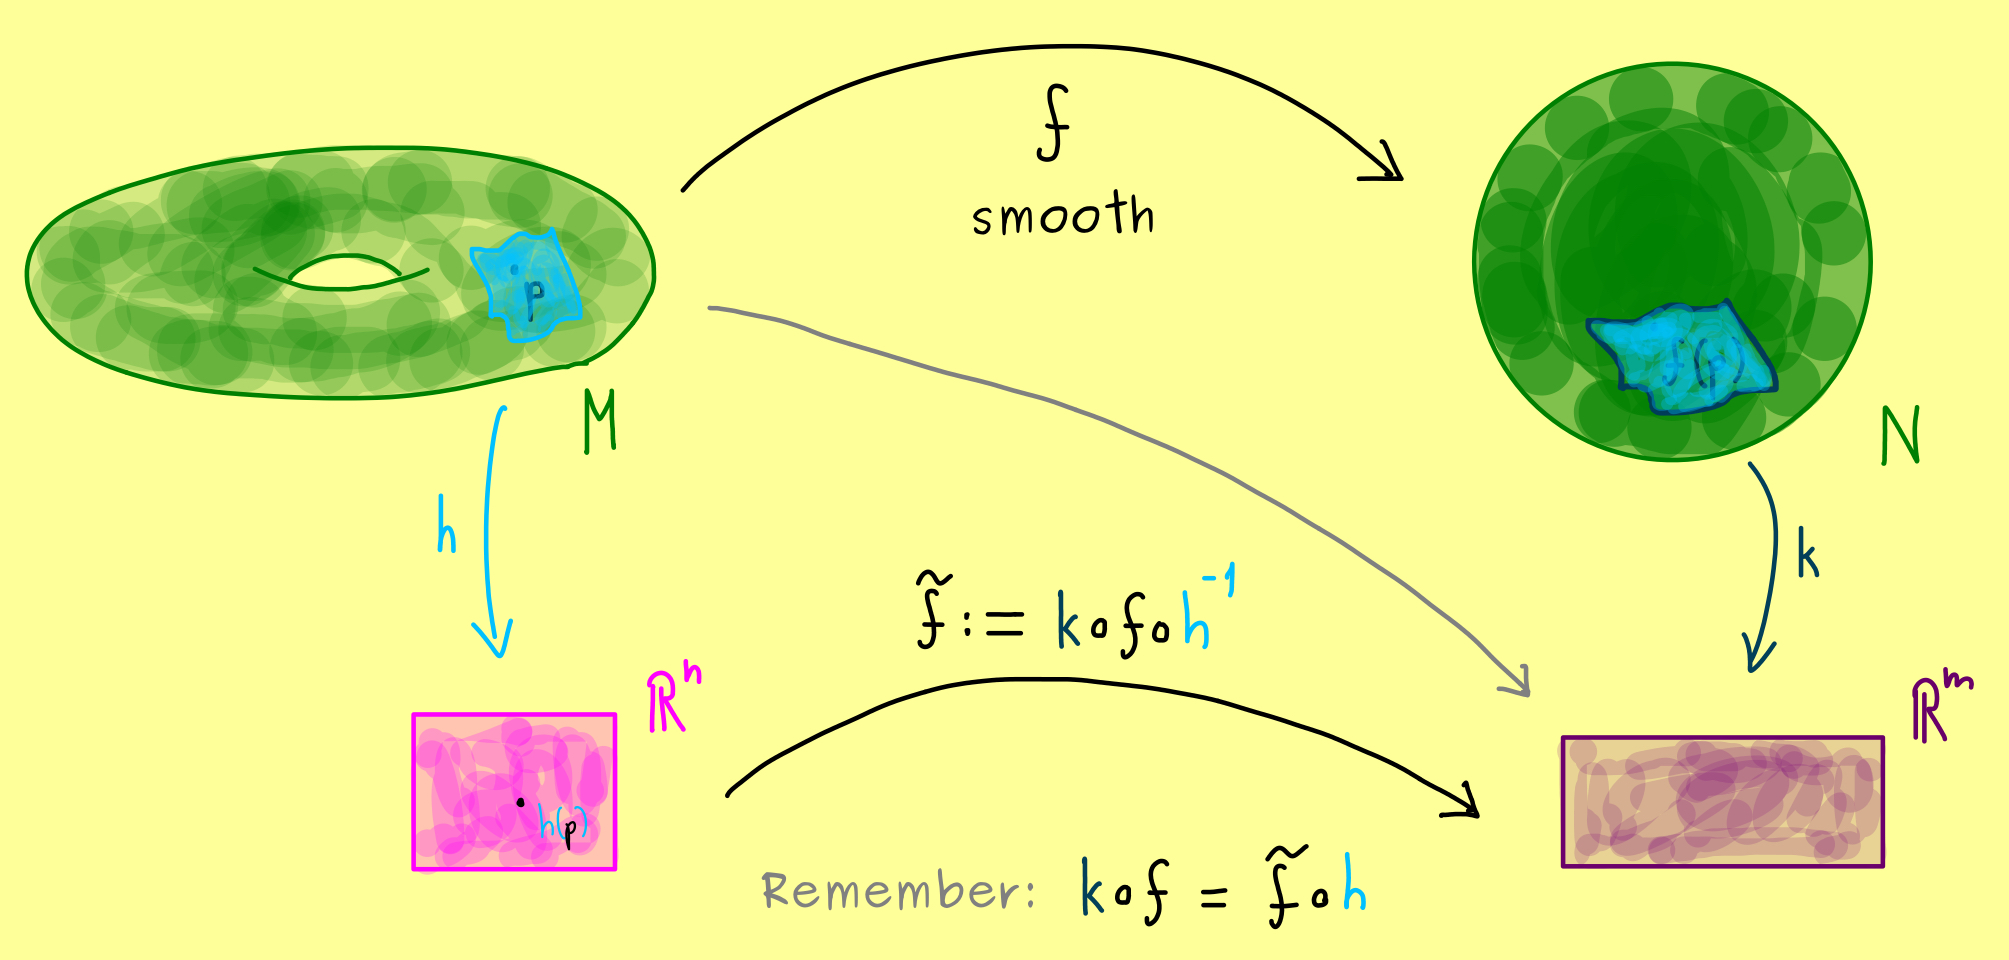
\includegraphics[width=0.8\textwidth]{Figs/differential_in_local_charts.jpeg}
    \caption{Differential in local charts}
\end{figure}


% * * * * * * * * * * * * * * * * * * * * * * * *
% * * * * * * * * * * * * * * * * * * * * * * * *
% * * * * * * * * * * * * * * * * * * * * * * * *
% * * * * * * * * * * * * * * * * * * * * * * * *
% * * * * * * * * * * * * * * * * * * * * * * * *
% * * * * * * * * * * * * * * * * * * * * * * * *
% * * * * * * * * * * * * * * * * * * * * * * * *

\chapter{Differential (example)}

We have previously defined the map $h_* : T_pM \to \mathbb{R}^n$ as $h_*([\gamma]_{\sim}) = (h \circ \gamma)'(0)$. \\
We have seen that $df_p([\gamma]_{\sim}) = [f \circ \gamma]_{\sim}$, and if the range of $f$ is a submanifold, then $df_p([\gamma]_{\sim}) = (f \circ \gamma)'(0)$. \\


Recall: for \( p \in M \) and $(U, h)$ the coordinate basis $\{ \partial_1, \ldots, \partial_n \}$ of $T_pM$ with respect to $(U, h)$
is given by $(\partial_1, \ldots, \partial_n)$ where $\partial_j := \varphi_*(e_j) = d\varphi_{h(p)}(e_j)$. \\ 

Directional derivative: \\
Let $f : M \to \mathbb{R}$ be a smooth map and $p \in M$. \\
In general, $df_p([\gamma]_{\sim})$ gives us a directional derivative. Then for partial derivatives $\partial_j f(p)$ we have $\tilde{\gamma}(t) = h(p) + t * e_j$ and \\
\begin{align*}
    \partial_j f(p) &:= df_p(\partial_j) \\
    &= df_p(d\varphi_{h(p)}(e_j)) \\
    &= [f \circ \varphi \circ \tilde{\gamma}]_{\sim} \\
    &= (f \circ \varphi \circ \tilde{\gamma})'(0) \\
    &= J_{f \circ \varphi}(h(p)) \cdot \tilde{\gamma}'(0) = \frac{\partial (f \circ \varphi)}{\partial x_j}(h(p))
\end{align*}



% * * * * * * * * * * * * * * * * * * * * * * * *
% * * * * * * * * * * * * * * * * * * * * * * * *
% * * * * * * * * * * * * * * * * * * * * * * * *
% * * * * * * * * * * * * * * * * * * * * * * * *
% * * * * * * * * * * * * * * * * * * * * * * * *
% * * * * * * * * * * * * * * * * * * * * * * * *
% * * * * * * * * * * * * * * * * * * * * * * * *

\chapter{Ricci calculus / Tensor calculus}

In Ricci calculus, we are calulating in the coordinates of a parametrization of a manifold. \\
Moreover, the poisition of indices in the notation is important (superscript indices are contravariant and subscript indices are covariant). \\

\begin{center} 
\begin{tabular}{|m{0.5\textwidth}|m{0.5\textwidth}|}
    \hline
    \multicolumn{1}{|c|}{\textbf{Our Language}} & \multicolumn{1}{c|}{\textbf{Ricci Calculus}} \\ 
    \hline
    components of a given chart $(U, h), h : U \to \mathbb{R}^n$ 
    & $h^j : U \to \mathbb{R}$ coordinates, or simply: $x^1, \ldots, x^n$ 
    \\ 
    \hline
    coordinate basis of $T_pM$: $\partial_j := \varphi_*(e_j)$
    & $\frac{\partial}{\partial x^1}, \ldots, \frac{\partial}{\partial x^n}$ 
    \\
    \hline
    tangent vector $[\gamma]_{\sim} \in T_pM$: $v_1 \partial_1 + \ldots + v_n \partial_n$
    & $v^1 \frac{\partial}{\partial x^1} + \ldots + v^n \frac{\partial}{\partial x^n} := v^j \frac{\partial}{\partial x^j}$ \\ &
    (Einsteins summation convention) ($\sum_{j=1}^{n} v^j \frac{\partial}{\partial x^j}$)
    \\
    \hline
    Inner product on $T_pM$: $\langle v, w\rangle \in \mathbb{R}$
    & $v^j g_{jk} w^k \in \mathbb{R}$ (metric tensor $g_{jk}$)
    \\
    \hline
\end{tabular}
\end{center}

We will deep dive later to the meaning of contravariant and covariant vectors, but for now:
\begin{itemize}
    \item Tangent vector is called contravariant vector in Ricci calculus.
\end{itemize}

\begin{definition}{\textbf{Contravariant vector}} \\
    A contravariant vector is a vector that transforms according to the rule: \\
    \begin{equation*}
        v^j \frac{\partial}{\partial x^j} \quad \text{where} \quad v^j \in \mathbb{R}
    \end{equation*}
\end{definition}

\begin{definition}{\textbf{Covariant vector}} \\
    A covariant vector is a vector that transforms according to the rule: \\
    \begin{equation*}
        v_j dx^j \quad \text{where} \quad v_j \in \mathbb{R}
    \end{equation*}
\end{definition}

Dual to a contravariant vector: $v_j dx^j$\\
For exmaple, the one-form for a vector in the tangent space: \\
In our language, $dx_j(\partial_k) = \delta_{jk}$, where $\delta_{jk}$ is the Kronecker delta.\\
In Ricci calculus, $dx^j(\frac{\partial}{\partial x^k}) = \delta^j_k$.



% * * * * * * * * * * * * * * * * * * * * * * * *
% * * * * * * * * * * * * * * * * * * * * * * * *
% * * * * * * * * * * * * * * * * * * * * * * * *
% * * * * * * * * * * * * * * * * * * * * * * * *
% * * * * * * * * * * * * * * * * * * * * * * * *
% * * * * * * * * * * * * * * * * * * * * * * * *
% * * * * * * * * * * * * * * * * * * * * * * * *

\chapter{Alternating k-forms}

\begin{definition}{\textbf{Dual Space (of a tangent space)}} \\
    Let \( M \) be an n-dimensional smooth manifold. \\
    The dual space of the tangent space of \( M \) at \( p \) is defined as
    \begin{equation*}
        T_p^*M := (T_pM)^* = \{ \alpha : T_pM \to \mathbb{R} \quad | \quad \alpha \quad \text{is linear} \}
    \end{equation*}
\end{definition}

For example, the one-form $dx_{j,p} : T_pM \to \mathbb{R}$ is defined as $dx_{j,p}(\partial_k) = \delta_{jk}$.

\begin{definition}{\textbf{Differential form}} \\
    A differential form on a smooth manifold \( M \) is a map $\omega$ defined on $M$ such that for each $p \in M$,
    $\omega(p)$ is a linear map $\omega_p : T_pM \to \mathbb{R}$.
\end{definition}

An example for a differential form is the one-form: $dx_j : p \mapsto dx_{j,p} \in T_p^*M$.

\begin{definition}{\textbf{k-linear (multilinear) map}} \\
    A map $f : V_1 \times \ldots \times V_k \to W$ is called k-linear if it is linear in each argument. \\ 
    That is, for each $i \in \{1, \ldots, k\}$, \\
    $f(v_1, \ldots, v_{i-1}, \lambda v_i + \mu v_i', v_{i+1}, \ldots, v_k) = \lambda f(v_1, \ldots, v_{i-1}, v_i, v_{i+1}, \ldots, v_k) + \mu f(v_1, \ldots, v_{i-1}, v_i', v_{i+1}, \ldots, v_k)$.
\end{definition}

\begin{definition}{\textbf{k-form}} \\
    Let \(V \) be a vector space. 
    A k-form on \( V \) is a k-linear map $\omega : V^k \to \mathbb{R}$.
\end{definition}

For exmaple, any inner product on a vector space \( V \) is a 2-form on \( V \) (bilinear form).

\begin{definition}{\textbf{Alternating k-form on $V$}} \\
    A k-form $\omega$ on \( V \) is called alternating if one of those conditions hold:
    \begin{itemize}
        \item $\omega(v_1, \ldots, v_k) = 0$ if $v_i = v_j$ for some $i \neq j$.
        \item $\omega(v_{\sigma(1)}, \ldots, v_{\sigma(k)}) = \text{sgn}(\sigma) \cdot \omega(v_1, \ldots, v_k)$ for each permutation $\sigma$ of $\{1, \ldots, k\}$. \\
            For example, $\omega(v_2, v_1, v_3) = -\omega(v_1, v_2, v_3)$.
        \item $\omega(v_1, \ldots, v_k) = 0$ if $v_i = \sum_{j=1}^{k} \lambda_j v_j$ for some $\lambda_j \in \mathbb{R}$ (linearly dependent vectors).
    \end{itemize}
\end{definition}

\begin{definition}{\textbf{$Alt^k(V)$}} \\
    Let \( V \) be a vector space. \\ 
    \begin{align*}
        Alt^k(V) &:= \{ \alpha : V^k \to \mathbb{R} \quad | \quad \omega \quad \text{is k-linear and alternating} \}
    \end{align*}
\end{definition}

Examples: 
\begin{itemize}
    \item $det \in Alt^n(\mathbb{R}^n)$ is an alternating n-form on $\mathbb{R}^n$.
    \item $Alt^1(V) = { \alpha : V \to \mathbb{R} \quad | \quad \alpha \quad \text{is linear} } = V^*$ is the dual space of \( V \).
    \item $Alt^0(V) = \mathbb{R}$.
\end{itemize}


% * * * * * * * * * * * * * * * * * * * * * * * *
% * * * * * * * * * * * * * * * * * * * * * * * *
% * * * * * * * * * * * * * * * * * * * * * * * *
% * * * * * * * * * * * * * * * * * * * * * * * *
% * * * * * * * * * * * * * * * * * * * * * * * *
% * * * * * * * * * * * * * * * * * * * * * * * *
% * * * * * * * * * * * * * * * * * * * * * * * *

\chapter{Wedge Product}

\begin{definition}{\textbf{Wedge product}} \\
    Let \( V \) be a vector space and \( \alpha \in Alt^k(V) \) and \( \beta \in Alt^s(V) \). \\
    The wedge product \( \wedge : Alt^k(V) \times Alt^s(V) \to Alt^{k+s}(V) \) is defined as
    \begin{align*}
        \wedge(\alpha, \beta) &\to \alpha \wedge \beta : V^{k+l} \to \mathbb{R} \quad \text{defined as} \\
        \alpha \wedge \beta(v_1, \ldots, v_{k+s}) &= \frac{1}{k! \cdot s!} \sum_{\sigma \in S_{k+s}} \text{sgn}(\sigma) \cdot \alpha(v_{\sigma(1)}, \ldots, v_{\sigma(k)}) \cdot \beta(v_{\sigma(k+1)}, \ldots, v_{\sigma(k+s)})
    \end{align*}
\end{definition}

Examples: 
\begin{itemize}
    \item $\alpha, \beta \in Alt^1(V) = V^*$. Then $\alpha \wedge \beta \in Alt^2(V)$, is a 2-form on \( V \) that is defined 
    as $\alpha \wedge \beta(v_1, v_2) = \alpha(v_1) \cdot \beta(v_2) - \alpha(v_2) \cdot \beta(v_1)$.
    
    
    \item $\alpha , \beta \in Alt^1(\mathbb{R}^3), \quad 
    \alpha ( \begin{pmatrix}
        x1 \\ x2 \\ x3
    \end{pmatrix}) = x1, \quad
    \beta ( \begin{pmatrix}
        x1 \\ x2 \\ x3
    \end{pmatrix}) = x2$. \\
    Then $\alpha \wedge \beta \in Alt^2(\mathbb{R}^3)$ is defined as
    \begin{align*}
        \alpha \wedge \beta ( \begin{pmatrix}
            x1 \\ x2 \\ x3
        \end{pmatrix}, \begin{pmatrix}
            y1 \\ y2 \\ y3
        \end{pmatrix}) &=  x1 \cdot y2 - y1 \cdot x2 = 
        \langle 
        \begin{pmatrix}
            x1 \\ x2 \\ x3
        \end{pmatrix}
        ,
        \begin{pmatrix}
            0 & 1 & 0 \\
            -1 & 0 & 0 \\
            0 & 0 & 0 \\
        \end{pmatrix}
        \begin{pmatrix}
            y1 \\ y2 \\ y3
        \end{pmatrix}
        \rangle
    \end{align*}

    and the matrix $\begin{pmatrix}
        0 & 1 & 0 \\
        -1 & 0 & 0 \\
        0 & 0 & 0 \\
    \end{pmatrix}$ is the matrix identified with the 2-form $\alpha \wedge \beta$.
\end{itemize}

\paragraph{Properties of the wedge product:}
\begin{enumerate}
    \item Anticommutative: $\alpha \wedge \beta = (-1)^{k \cdot s} \cdot \beta \wedge \alpha$.
    \item Bilinear:
        \begin{itemize}
            \item $(\alpha + \beta) \wedge \gamma = \alpha \wedge \gamma + \beta \wedge \gamma$.
            \item $\lambda (\cdot \alpha) \wedge \beta = \lambda \cdot (\alpha \wedge \beta)$.
        \end{itemize}
    \item Associative: $(\alpha \wedge \beta) \wedge \gamma = \alpha \wedge (\beta \wedge \gamma)$.
    \item Pullback: for a linear map $f : W \to V$, and $\alpha \in Alt^k(V)$, $(f^* \alpha)(w_1, \ldots, w_k) = \alpha(f(w_1), \ldots, f(w_k))$. \\
        $f^*(\alpha \wedge \beta) = f^* \alpha \wedge f^* \beta$.
\end{enumerate}


The wedge product of two vectors, \(\mathbf{u}\) and \(\mathbf{v}\), represented as \(\mathbf{u} \wedge \mathbf{v}\), 
can be interpreted geometrically as the oriented area of the parallelogram spanned by these two vectors. 
The orientation is significant because swapping the vectors reverses the sign of the resulting area.

Mathematically, if \(\mathbf{u} = ai + bj\) and \(\mathbf{v} = ci + dj\), where i and j are basis vectors, then the wedge product is defined as:

\begin{align*}
    i \wedge i = 0, \quad j \wedge j = 0
\end{align*}

\begin{align*}
    0 = (i + j) \wedge (i + j) = i \wedge i + i \wedge j + j \wedge i + j \wedge j = i \wedge j + j \wedge i \Rightarrow i \wedge j = -j \wedge i
\end{align*}

\begin{align*}
\mathbf{u} \wedge \mathbf{v} &= (ai + bj) \wedge (ci + dj) \\
&= ai \wedge ci + ai \wedge dj + bj \wedge ci + bj \wedge dj \\
&= ac i \wedge i + ad i \wedge j + bc j \wedge i + bd j \wedge j \\
&= (ad - bc) i \wedge j
\end{align*}



% * * * * * * * * * * * * * * * * * * * * * * * *
% * * * * * * * * * * * * * * * * * * * * * * * *
% * * * * * * * * * * * * * * * * * * * * * * * *
% * * * * * * * * * * * * * * * * * * * * * * * *
% * * * * * * * * * * * * * * * * * * * * * * * *
% * * * * * * * * * * * * * * * * * * * * * * * *
% * * * * * * * * * * * * * * * * * * * * * * * *

\chapter{Differential forms}

\begin{definition}{\textbf{k-form on the manifold}} \\
    A k-form on a smooth manifold \( M \) is a map 
    \begin{align*}
        \omega &: M \to \cup_{p \in M} Alt^k(T_pM) \\
        p &\mapsto \omega_p = w(p) \in Alt^k(T_pM)
    \end{align*}
\end{definition}

\bigbreak

We also define: $\omega \wedge \eta : M \to \cup_{p \in M} Alt^{k+s}(T_pM)$ as $(\omega \wedge \eta)_p := \omega_p \wedge \eta_p$. 
\medbreak
For any smooth map $f : M \to N$, we define $f^* \omega : M \to \cup_{p \in M} Alt^k(T_pM)$ as \\
$(f^* \omega)(p) := (df_p)^* \omega_{p}$.

\paragraph{Basis elements}: \\
Recall, For a chart $(U, h)$ of $M$ at $p$, the coordinate basis of $T_pM$ is $( \partial_1, \ldots, \partial_n )$, with $\partial_j = \varphi_*(e_j) = d\varphi_{h(p)}(e_j)$. \\
Then, the dual basis of $(T_pM)* = Alt^1(T_pM)$ is $( dx_p^1, \ldots, dx_p^n )$ where $dx_p^j(\partial_k) = \delta_k^j$.

\begin{definition}\textbf{Basis elements of k-forms} \\
    Let $dx_p^1, \ldots, dx_p^n$ be the dual basis of $T_pM$ at $p$. \\
    The basis elements of $Alt^k(T_pM)$ are defined as
    \begin{align*}
        &(dx_p^{\mu_1} \wedge \ldots \wedge dx_p^{\mu_k})_{\mu_1 < \mu_2 < \ldots < \mu_k} : T_pM^k \to \mathbb{R} 
    \end{align*}
\end{definition}

Example: $dim(M) = 3$, then the basis elements of $Alt^2(T_pM)$ are $(dx_p^1 \wedge dx_p^2, dx_p^1 \wedge dx_p^3, dx_p^2 \wedge dx_p^3)$.

\bigbreak

Conclusion: \\
Each k-form on a manifold M can locally be written as a linear combination of the basis elements of $Alt^k(T_pM)$:
\begin{equation*}
    \omega(p) = \sum_{\mu_1 < \ldots < \mu_k} \omega_{\mu_1, \ldots, \mu_k}(p) \cdot dx_p^{\mu_1} \wedge \ldots \wedge dx_p^{\mu_k}
\end{equation*}
Each $\omega_{\mu_1, \ldots, \mu_k} : U \to \mathbb{R}$ is called a component function of $\omega$ in the chart $(U, h)$.

\begin{definition}{\textbf{Differentible k-form on M}} \\
    A k-form $\omega$ on a smooth manifold \( M \) is called differentiable if for each chart $(U, h)$ of \( M \), 
    the component functions $\omega_{\mu_1, \ldots, \mu_k}$ are differentiable. \\
    We denote the set of all differentiable k-forms on \( M \) as \( \Omega^k(M) \).
    We define \( \Omega^0(M) = C^{\infty}(M) \).
\end{definition}



% * * * * * * * * * * * * * * * * * * * * * * * *
% * * * * * * * * * * * * * * * * * * * * * * * *
% * * * * * * * * * * * * * * * * * * * * * * * *
% * * * * * * * * * * * * * * * * * * * * * * * *
% * * * * * * * * * * * * * * * * * * * * * * * *
% * * * * * * * * * * * * * * * * * * * * * * * *
% * * * * * * * * * * * * * * * * * * * * * * * *

\chapter{Examples of differential forms}

M = $\mathbb{R}^2$ , $\partial_1 = \frac{\partial}{\partial x} = \begin{pmatrix} 1 \\ 0 \end{pmatrix}$, $\partial_2 = \frac{\partial}{\partial y} = \begin{pmatrix} 0 \\ 1 \end{pmatrix}$, 
$dx_p^1 = \begin{pmatrix} 1 & 0 \end{pmatrix}$, $dx_p^2 = \begin{pmatrix} 0 & 1 \end{pmatrix}$ \\
\begin{align*}
    dx_p^1 \wedge dx_p^2 ( \begin{pmatrix} a_{1,1} \\ a_{2,1} \end{pmatrix}, \begin{pmatrix} a_{1,2} \\ a_{2,2} \end{pmatrix}) &=  
    \sum_{\sigma \in S_2} \text{sgn}(\sigma) \cdot dx_p^1(\begin{pmatrix} a_{1, \sigma(1)} \\ a_{2, \sigma(1)} \end{pmatrix}) \cdot dx_p^2(\begin{pmatrix} a_{1, \sigma(2)} \\ a_{2, \sigma(2)} \end{pmatrix}) 
    \\&= \sum_{\sigma \in S_2} \text{sgn}(\sigma) \cdot a_{1, \sigma(1)} \cdot a_{2, \sigma(2)} 
    \\&= det \begin{pmatrix} a_{1,1} & a_{1,2} \\ a_{2,1} & a_{2,2} \end{pmatrix}
\end{align*}

In general for $\mathbb{R}^n$, $dx_p^{\mu_1} \wedge \ldots \wedge dx_p^{\mu_k} ( \begin{pmatrix} a_{1,1} \\ \vdots \\ a_{n,1} \end{pmatrix}, \ldots, \begin{pmatrix} a_{1,k} \\ \vdots \\ a_{n,k} \end{pmatrix}) = det \begin{pmatrix} a_{1,1} & \ldots & a_{1,k} \\ \vdots & \ddots & \vdots \\ a_{n,1} & \ldots & a_{n,k} \end{pmatrix}$

\bigbreak

M = $\mathbb{R}^2$, $\varphi : (r, \theta) \to \mathbb{R}^2$, $\varphi(r, \theta) = \begin{pmatrix} r \cdot cos(\theta) \\ r \cdot sin(\theta) \end{pmatrix}$ \\
$\partial_1(r, \theta) = \frac{\partial \varphi }{\partial r}(r, \theta) = \begin{pmatrix} cos(\theta) \\  sin(\theta) \end{pmatrix}$, 
$\partial_2(r, \theta) = \frac{\partial  \varphi}{\partial \theta}(r, \theta) = \begin{pmatrix} -r \cdot sin(\theta) \\ r \cdot cos(\theta) \end{pmatrix}$ \\
The corresponding dual basis is $dr_p = \begin{pmatrix} cos(\theta) & sin(\theta) \end{pmatrix}$, $d\theta_p = \frac{1}{r} \begin{pmatrix} - \cdot sin(\theta) & \cdot cos(\theta) \end{pmatrix}$ \\
for $p = (x, y)$, $dr_p = \begin{pmatrix} \frac{x}{\sqrt{x^2 + y^2}} & \frac{y}{\sqrt{x^2 + y^2}} \end{pmatrix}$, $d\theta_p = \begin{pmatrix} - \frac{y}{x^2 + y^2} & \frac{x}{x^2 + y^2} \end{pmatrix}$ \\
Then $(dr_p \wedge d\theta_p) (e_1, e_2) = dr_p(e_1) \cdot d\theta_p(e_2) - dr_p(e_2) \cdot d\theta_p(e_1) = \frac{1}{r} (\cos^2(\theta) + \sin^2(\theta)) = \frac{1}{r}$

% * * * * * * * * * * * * * * * * * * * * * * * *
% * * * * * * * * * * * * * * * * * * * * * * * *
% * * * * * * * * * * * * * * * * * * * * * * * *
% * * * * * * * * * * * * * * * * * * * * * * * *
% * * * * * * * * * * * * * * * * * * * * * * * *
% * * * * * * * * * * * * * * * * * * * * * * * *
% * * * * * * * * * * * * * * * * * * * * * * * *

\chapter{Orientable manifolds}

For example. $\mathbb{R}^n$ with basis $(e_1, \ldots, e_n)$ is oriented by the basis $(e_1, \ldots, e_n)$. \\
For change of basis matrix $T_{C \leftarrow B}$, 
$det(T_{C \leftarrow B}) > 0$ means that the basis $C$ is positively oriented with respect to the basis $B$, 
and $det(T_{C \leftarrow B}) < 0$ means that the basis $C$ is negatively oriented with respect to the basis $B$. \\
\medbreak
Thus, there are two equivalence classes of bases: positively and negatively oriented bases with respect to the standard basis. \\

\begin{definition}{\textbf{Orientation in vector spaces}} \\
    An orientation $(V, or)$ is a tuple of V finite-dimensional vector space and a choice of an equivalence class of bases. \\
\end{definition}

Let M be an n-dimensional smooth manifold, and $p \in M$. \\
Let \(U, h\) be a chart of \(M\) at \(p\), and $\varphi_* : \mathbb{R}^n \to T_pM$ be the differential of the chart map, $e_j \to \partial_j^{h}(p)$. \\

\begin{definition}{\textbf{Orientable manifold}} \\
    A smooth manifold \( M \) is called orientable if there is a family of orientations for the tangent spaces $\{(T_pM, or_p)\}_{p \in M}$ such that
    $\forall p \in M, \exists (U,h) \quad \text{chart of} \quad M \quad \text{at} \quad p$ such that $\forall x \in U$: $(\partial_1^h(x), \ldots, \partial_n^h(x)) \in or x$.
\end{definition}

% * * * * * * * * * * * * * * * * * * * * * * * *
% * * * * * * * * * * * * * * * * * * * * * * * *
% * * * * * * * * * * * * * * * * * * * * * * * *
% * * * * * * * * * * * * * * * * * * * * * * * *
% * * * * * * * * * * * * * * * * * * * * * * * *
% * * * * * * * * * * * * * * * * * * * * * * * *
% * * * * * * * * * * * * * * * * * * * * * * * *

\todo[inline]{complete the orientation section}
% \chapter{Alternative definitions for orientation}


% * * * * * * * * * * * * * * * * * * * * * * * *
% * * * * * * * * * * * * * * * * * * * * * * * *
% * * * * * * * * * * * * * * * * * * * * * * * *
% * * * * * * * * * * * * * * * * * * * * * * * *
% * * * * * * * * * * * * * * * * * * * * * * * *
% * * * * * * * * * * * * * * * * * * * * * * * *
% * * * * * * * * * * * * * * * * * * * * * * * *

\chapter{Riemannian metrics}

% * * * * * * * * * * * * * * * * * * * * * * * *
% * * * * * * * * * * * * * * * * * * * * * * * *
% * * * * * * * * * * * * * * * * * * * * * * * *
% * * * * * * * * * * * * * * * * * * * * * * * *
% * * * * * * * * * * * * * * * * * * * * * * * *
% * * * * * * * * * * * * * * * * * * * * * * * *
% * * * * * * * * * * * * * * * * * * * * * * * *

% \chapter{Examples for Riemannian Manifolds}

% * * * * * * * * * * * * * * * * * * * * * * * *
% * * * * * * * * * * * * * * * * * * * * * * * *
% * * * * * * * * * * * * * * * * * * * * * * * *
% * * * * * * * * * * * * * * * * * * * * * * * *
% * * * * * * * * * * * * * * * * * * * * * * * *
% * * * * * * * * * * * * * * * * * * * * * * * *
% * * * * * * * * * * * * * * * * * * * * * * * *

% \chapter{Canonical Volume Form}




% * * * * * * * * * * * * * * * * * * * * * * * * 
% * * * * * * * * * * * * * * * * * * * * * * * * 
% * * * * * * * * * * * * * * * * * * * * * * * * 
% * * * * * * * * * * * * * * * * * * * * * * * * 
% * * * * * * * * * * * * * * * * * * * * * * * * 
% * * * * * * * * * * * * * * * * * * * * * * * * 
% * * * * * * * * * * * * * * * * * * * * * * * * 
% * * * * * * * * * * * * * * * * * * * * * * * * 
% * * * * * * * * * * * * * * * * * * * * * * * * 
% * * * * * * * * * * * * * * * * * * * * * * * * 
% * * * * * * * * * * * * * * * * * * * * * * * * 
% * * * * * * * * * * * * * * * * * * * * * * * * 
% * * * * * * * * * * * * * * * * * * * * * * * * 
% * * * * * * * * * * * * * * * * * * * * * * * * 
% * * * * * * * * * * * * * * * * * * * * * * * * 
% * * * * * * * * * * * * * * * * * * * * * * * * 
% * * * * * * * * * * * * * * * * * * * * * * * * 
% * * * * * * * * * * * * * * * * * * * * * * * * 
% * * * * * * * * * * * * * * * * * * * * * * * * 

\end{document}